%% USPSC-Apendice.tex
% ---
% Inicia os apêndices
% ---

\begin{apendicesenv}
	% Imprime uma página indicando o início dos apêndices
	\partapendices
	\chapter{Linked Open Social Data for Scientific Benchmarking (diagrams)}\label{ap:losd}

	In this document we provide diagrams
	for the social protocols in the Linked Open Social Database:
	Facebook, Twitter, IRC, Email, ParticipaBR, Cidade Democrática and AA.
	Each social protocol diagram was broken in two, one presents the relations
	among main classes (blue nodes) and data types (orange nodes),
	the other presents metadata for the
	snapshots.
	Every class instance is related to the snapshot instance
	by the triple \textttt{class\_uri po:snapshot snapshot\_uri}.
	Such triples are omitted for simplicity.
	Due to the large number of relations, the rendering of diagrams are
	automatized and displays some overlaps.
	Even so, the images are useful for grasping what is in the current
	database and for conducting explorations.
	Edges in the diagrams have:
	\begin{itemize}
		\item green color if representing an OWL existential
			class restriction (all individuals from the class present at least one triple with
				    the property as predicate);
			    \item inverted nip if representing an OWL universal class
				    restriction (all individuals presenting triples with the
								property as predicate are from the class);
							\item full edges (non-dashed) if representing a functional property
								axiom (there is at most one triple with the property as the
											    predicate for each individual).
	\end{itemize}

	% \textheight = 100pt
	% \pdfpageheight 300pt
	Furthermore, this document ends with two sets of tables, one with
	references for snapshot groups, such as wikipedia or
	contact links, 
	the other with 
	counts of
	triples, participants, edges/interactions/relations and characters.


	\section{Facebook data}
	Each Facebook snapshot is yield by either an user, from which the
	friends constitute a friendship network, or a group, which participants
	can yield friendship and interaction networks and posts information with
	text and some metadata.
	Further information is found on the following diagrams, the tables on
	the end of this document or in the main document of this
	article~\cite{losd}.

	% 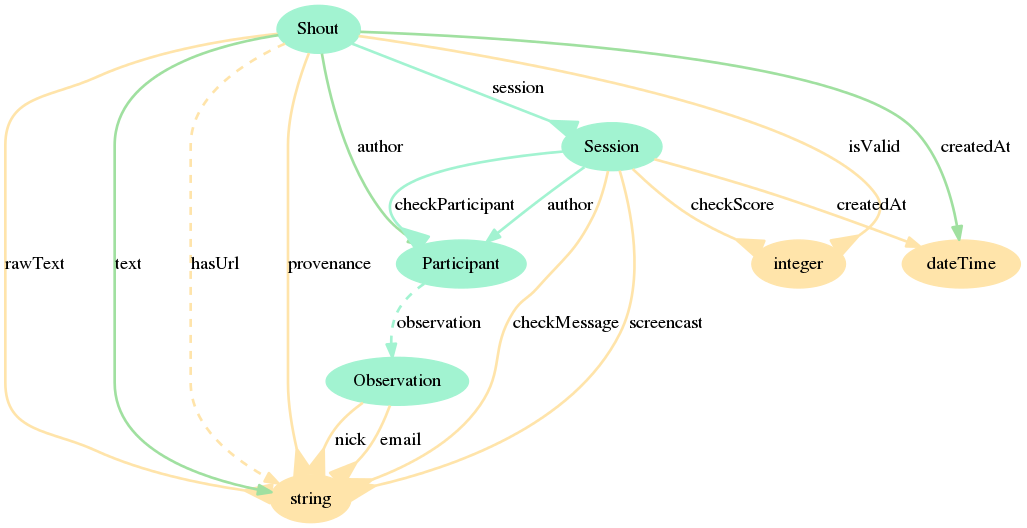
\includepdf{ontologies/aairc.ttl/draw.pdf}
	\incgraph[
		overlay={\node[red,below right] at (page.north west) {\Huge Facebook};}
		      paper=graphics
		      ][scale=.6]{ontologies/facebook-legacy-Auricultura10042013Friendship.ttl/draw.png}

		      \textheight = 2in
		      \pdfpageheight 5in
		      \incgraph[
			      overlay={\node[red,below right] at (page.north west) {\Huge Facebook};}
				    paper=graphics
				    ][scale=.5]{ontologies/facebook-legacy-Auricultura10042013Meta.ttl/draw.png}

				    \section{Twitter data}
				    Each Twitter snapshot is yield by a hashtag.
				    Retweets (\textttt{po:retweetOf} are usually considered the interactions between users.
				    The database present also \textttt{po:replyTo} and \textttt{po:userMention}
				    which might be useful in understanding the networking.
				    Further information is found on the following diagrams, the tables on
				    the end of this document or in the main document of this
				    article~\cite{losd}.

				    \incgraph[
					    overlay={\node[red,below right] at (page.north west) {\Huge
						Twitter };}
						    paper=graphics
						    ][scale=.5]{ontologies/twitter-legacy-arenaNETmundialTweet00000.ttl/draw.png}

						    \incgraph[
							    overlay={\node[red,below right] at (page.north west) {\Huge Twitter};}
								  paper=graphics
								  ][scale=.7]{ontologies/twitter-legacy-arenaNETmundialMeta.ttl/draw.png}

								  \section{IRC data}
								  Each IRC snapshot is yield by an IRC channel.
								  IRC messages are either server messages (e.g. join and exit)
								  marked with \textttt{po:systemMessage true} and having an \textttt{po:impliedUser user\_uri},
								  or user messages, which yield interactions through \textttt{po:directedTo} and \textttt{po:mentions} properties.
								  Text messages without the user names are delivered through the \textttt{po:cleanText} property.
								  Further information is found on the following diagrams, the tables on
								  the end of this document or in the main document of this
								  article~\cite{losd}.
								  \incgraph[
									  overlay={\node[red,below right] at (page.north west) {\Huge IRC};}
										paper=graphics
										][scale=.7]{ontologies/irc-legacy-hackerspace-cpsLog00000.ttl/draw.png}
										\incgraph[
											overlay={\node[red,below right] at (page.north west) {\Huge IRC};}
											      paper=graphics
											      ][scale=.6]{ontologies/irc-legacy-hackerspace-cpsMeta.ttl/draw.png}

											      \section{Email data}
											      Each email snapshot is yield by an Email list.
											      Interactions are yield through \textttt{po:replyTo} relations
											      although \textttt{po:to} and \textttt{po:cc} might also be considered.
											      The email body is given by \textttt{po:text} relations while
											      \textttt{po:cleanText} links to text with lines removed where they are
											      trivially from previous messages or computer code.
											      Further information is found on the following diagrams, the tables on
											      the end of this document or in the main document of this
											      article~\cite{losd}.
											      \incgraph[
												      overlay={\node[red,below right] at (page.north west) {\Huge Email};}
													    paper=graphics
													    ][scale=.4]{ontologies/email-legacy-linux.audio.devel1-20000Email00000.ttl/draw.png}
													    \textheight = 3in
													    \pdfpageheight 6in
													    \incgraph[
														    overlay={\node[red,below right] at (page.north west) {\Huge Email};}
															  paper=graphics
															  ][scale=.5]{ontologies/email-legacy-linux.audio.devel1-20000Meta.ttl/draw.png}

															  \section{ParticipaBR data}
															  The ParticipaBR snapshot is yield by a data dump donated by the system
															  administrators of the federal portal of social participation ParticipaBR.
															  Articles can have parent articles (\textttt{po:parent}), be step of a
															  collection of articles (\textttt{po:stepOf}) and be a mediation of other
															  articles (\textttt{po:mediationOf}).
															  Interactions are yield by comments which are \textttt{po:replyTo} other
															  comments or which are made directly to an article.
															  This snapshot holds also friendship structures.
															  The language used is mainly Brazilian Portuguese, but English and
															  Spanish are also incident.
															  Due to the higher complexity of the diagram, an additional figure is
															  given rendered with another layout algorithm.
															  Further information is found on the following diagrams, the tables on
															  the end of this document or in the main document of this
															  article~\cite{losd}.
															  \incgraph[
																  overlay={\node[red,below right] at (page.north west) {\Huge
																      ParticipaBR};}
																	  paper=graphics
																	  ][scale=.5]{ontologies/participabr.ttl/draw.png}
																	  \incgraph[
																		  overlay={\node[red,below right] at (page.north west) {\Huge
																		      ParticipaBR};}
																			  paper=graphics
																			  ][scale=.7]{ontologies/participabr.ttl/draw_circo.png}
																			  \incgraph[
																				  overlay={\node[red,below right] at (page.north west) {\Huge
																				      ParticipaBR};}
																					  paper=graphics
																					  ][scale=.7]{ontologies/participabrMeta.ttl/draw.png}

																					  \section{Cidade Democrática data}
																					  The Cidade Democrática snapshot is yield by a data dump donated by the system
																					  administrators of the civil society social participation portal Cidade
																					  Democrática.
																					  This snapshot holds a complex structure of both
																					  Topics/Inspirati-ons/Observatories/Supports/Competitions/Prizes
																					  and of State/City/Neighbor-hood/Place.
																					  The language used is mainly Brazilian Portuguese.
																					  Due to the higher complexity of the diagram, an additional figure is
																					  given rendered with another layout algorithm.
																					  Further information is found on the following diagrams, the tables on
																					  the end of this document or in the main document of this
																					  article~\cite{losd}.
																					  \incgraph[
																						  overlay={\node[red,below right] at (page.north west) {\Huge Cidade
																						      Democrática};}
																							  paper=graphics
																							  ][scale=.4]{ontologies/cidadedemocratica00000.ttl/draw.png}
																							  \textheight = 2in
																							  \pdfpageheight 5in
																							  \incgraph[
																								  overlay={\node[red,below right] at (page.north west) {\Huge Cidade
																								      Democrática};}
																									  paper=graphics
																									  ][scale=.4]{ontologies/cidadedemocratica00000.ttl/draw_circo.png}

																									  \incgraph[
																										  overlay={\node[red,below right] at (page.north west) {\Huge Cidade
																										      Democrática};}
																											  paper=graphics
																											  ][scale=.7]{ontologies/cidadedemocraticaMeta.ttl/draw.png}

																											  \section{AA data}
																											  The AA (Algorithmic Autoregulation) snapshots are yield by a data dump donated by the system
																											  administrators and by a mined IRC log.
																											  The system pursue simplicity and most of data consists of detached
																											  shouts with \textttt{po:text} and \textttt{po:author}.
																											  Further information is found on the following diagrams, the tables on
																											  the end of this document or in the main document of this
																											  article~\cite{losd}.
																											  \incgraph[
																												  overlay={\node[red,below right] at (page.north west) {\Huge AA};}
																													paper=graphics
																													][scale=.6]{ontologies/aairc.ttl/draw.png}
																													\textheight = 7in
%																													\pdfpageheight \foobar
																													\incgraph[
																														overlay={\node[red,below right] at (page.north west) {\Huge AA};}
																														      paper=graphics
																														      ][scale=.7]{ontologies/aaircMeta.ttl/draw.png}

																														      \section{Snapshot references}
																														      \label{sreferences}
																														      \pdfpageheight 10in
																														      \begin{table*}[h!]
\begin{center}\scriptsize
\caption{All the Facebook snapshots are either the result of individuals who downloaded
their data (and donated to the first author) or data downloaded from groups.
In the first case, it is senseless to present references. In the second
case, we present the group name and a link to a post in the group where
data and figures were delivered back to the group.}
\begin{tabular}{| l | p{9.9cm} |}\hline
\textbf{group name} & \textbf{url(s)} \\\hline
Adorno Nao Eh Enfeite & \url{https://www.facebook.com/groups/265217103529531/permalink/525654127485826/} \\\hline
Ativistas Da Inclusao Digital & \url{https://www.facebook.com/groups/423602557691243/permalink/525201037531394/} \\\hline
Ciencias Com Fronteiras & \url{https://www.facebook.com/groups/contraaexclusao/permalink/269103356558439/} \\\hline
Computer Art & \url{https://www.facebook.com/groups/computerart/permalink/259389137529870/} \\\hline
Coolmeia &  \url{https://www.facebook.com/groups/coolmeia/permalink/380091142098291/} , \url{https://www.facebook.com/groups/coolmeia/permalink/489757754464962/} \\\hline
Democracia Direta Ja & \url{https://www.facebook.com/groups/ddjbrasil/permalink/347023325397298/} \\\hline
Democracia Pura & \url{https://www.facebook.com/groups/democraciapura/permalink/310907215704321/} \\\hline
Economia & \url{https://www.facebook.com/groups/economa1/permalink/586007714743535/} \\\hline
Economia Criativa Digital & \url{https://www.facebook.com/groups/economiacriativadigital/permalink/438313682916103/} \\\hline
Educacoes E Aprendizagens XXI & \url{https://www.facebook.com/groups/geaxxi/permalink/433229973421182/} \\\hline
Latesfip & \url{https://www.facebook.com/groups/183557128478424/permalink/266610616839741/} \\\hline
Living Bridges Planet & \url{https://www.facebook.com/groups/livingbridgesplanet/permalink/352950408144951/} \\\hline
Mobilizacoes Culturais Interior SP & \url{https://www.facebook.com/groups/131639147005593/permalink/144204529082388/} \\\hline
Partido Pirata & \url{https://www.facebook.com/groups/partidopiratabrasil/permalink/10151409024509317/} \\\hline
Politicas Culturas Brasileiras & \url{https://www.facebook.com/groups/pcult/permalink/519626544747423/} \\\hline
Praca Popular & \url{https://www.facebook.com/groups/215924991863921/permalink/319279541528465/} \\\hline
Rede Tranzmidias & \url{https://www.facebook.com/groups/318333384951196/permalink/346658712118663/} \\\hline
Silicon Valley Global Network & \url{https://www.facebook.com/groups/109971182359978/permalink/589326757757749/} \\\hline
Solidarity Economy & \url{https://www.facebook.com/groups/9149038282/permalink/10151461945623283/} \\\hline
Study Group SNA & \url{https://www.facebook.com/groups/140630009439814/permalink/151470598355755/} \\\hline
Tecnoxamanismo &  \url{https://www.facebook.com/groups/505090906188661/permalink/733144993383250/} , \url{https://www.facebook.com/groups/505090906188661/permalink/733157380048678/} \\\hline
\end{tabular}\end{center}
\end{table*}




																														      \begin{table*}[h!]\scriptsize
																															      \begin{center}
																																      \caption{Different Twitter snapshots are yield by different hashtags. In this
																																      table we present each snapshot with the respective hashtag and a
																																      reference to the subject.}\label{tab:provenance}
																																      \begin{tabular}{| l || p{4cm} | p{4cm} | }\hline
																																	      \textbf{snapshot hashtag} & \textbf{observation} & \textbf{reference} \\\hline\hline
																																		      \#arenaNETmundial & a Brazilian discussion hub about free culture, democracy and the internet & \url{http://www.participa.br/netmundial} \\\hline
																																			  \#art & tweets with the generic hashtag \#art & \url{https://en.wikipedia.org/wiki/Art} \\\hline
																																			      \#ChennaiFloods & heavy rainfall generated by the annual northeast monsoon in November–December 2015 & \url{https://en.wikipedia.org/wiki/2015_South_Indian_floods} \\\hline
																																				  \#dilma & the 36th President of Brazil & \url{https://en.wikipedia.org/wiki/Dilma_Rousseff} \\\hline
																																				      \#ForaDilma & 2015-16 anti-government protests in Brazil & \url{https://en.wikipedia.org/wiki/2015-16_protests_in_Brazil} \\\hline
																																					  \#ForaCunha & 2015-16 anti-corruption protests in Brazil & \url{https://en.wikipedia.org/wiki/2015-16_protests_in_Brazil} \\\hline
																																					      \#fuck & tweets with the generic hashtag \#fuck & \url{https://en.wikipedia.org/wiki/Fuck} \\\hline
																																						  \#game & tweets with the generic hashtag \#game & \url{https://en.wikipedia.org/wiki/Game} \\\hline
																																						      \#god & tweets with the generic hashtag \#god & \url{https://en.wikipedia.org/wiki/God} \\\hline
																																							  \#MAMA2015 & the grand 2015 Mnet Asian Music Awards & \url{https://en.wikipedia.org/wiki/2015_Mnet_Asian_Music_Awards} \\\hline
																																							      \#music & tweets with the generic hashtag \#music & \url{https://en.wikipedia.org/wiki/Music} \\\hline
																																								  \#obama & the 44th President of the United States & \url{https://en.wikipedia.org/wiki/Barack_Obama} \\\hline
																																								      \#python & the Python programming language & \url{https://en.wikipedia.org/wiki/Python_(programming_language)} \\\hline
																																									  \#QuartaSemRacismoClubeSDV & an anti-racism netweaving & \url{https://twitter.com/hashtag/quartasemracismoclubesdv} \\\hline
																																									      \#science & tweets with the generic hashtag \#science & \url{https://en.wikipedia.org/wiki/Science} \\\hline
																																										  \#SnapDetremura & reference for Snapchat about a celebrated person & \url{https://twitter.com/detremura} \\\hline
																																      \end{tabular}\end{center}
																															      \end{table*}                    


																															      \begin{table*}[h!]\scriptsize
																																      \begin{center}
																																	      \caption{Different IRC snapshots are yield by different channels. In this
																																	      table we present each snapshot with the respective channel and a
																																	      reference to the subject.}\label{tab:provenance}
																																	      \begin{tabular}{| l || p{4cm} | p{4cm} | }\hline
																																		      \textbf{snapshot channel} & \textbf{observation} & \textbf{reference} \\\hline\hline
																																			      \#foradoeixo & a Brazilian network of culture related collectives & \url{https://pt.wikipedia.org/wiki/Fora_do_Eixo} \\\hline
																																				  \#hackerspace-cps & a hackerspace in Campinas, Brazil & \url{https://lhc.net.br/wiki/P%C3%A1gina_principal} \\\hline
																																				      \#hackerspaces-br & Brazilian hackerspaces channel & \url{https://garoa.net.br/wiki/Hackerspaces_Brasileiros} \\\hline
																																					  \#labmacambira & Brazilian channel for the labMacambira collective & \url{http://labmacambira.sourceforge.net/} \\\hline
																																	      \end{tabular}\end{center}
																																      \end{table*}                    

																																      \begin{table*}[h!]\scriptsize
																																	      \begin{center}
																																		      \caption{Different Email snapshots are yield by different email lists. In this
																																		      table we present each snapshot with the respective list and a
																																		      reference to the subject.}\label{tab:provenance}
																																		      \begin{tabular}{| p{4cm} || p{4cm} | p{4cm} | }\hline
																																			      \textbf{Gmane ID} & \textbf{observation} & \textbf{reference} \\\hline\hline
																																				      gmane.linux.audio.users & the Linux Audio Users & \url{http://linuxaudio.org} \\\hline
																																					  gmane.politics.organizations.me-tareciclagem & a network about technology and social transformation  & \url{https://metareciclagem.github.io} \\\hline
																																					      gmane.linux.audio.devel & the Linux Audio Developers & \url{http://lists.linuxaudio.org/listinfo/linux-audio-dev} \\\hline
																																						  gmane.comp.gcc.libstdc++.devel & the C++ standard library & \url{https://gcc.gnu.org/libstdc++/} \\\hline
																																		      \end{tabular}\end{center}
																																	      \end{table*}                    

																																	       \begin{table*}[h!]\scriptsize
																																		       \begin{center}
																																			       \caption{References for the snapshots of the detached instances
																																			       ParticipaBR, Cidade Democrática and AA.}\label{tab:provenance}
																																			       \begin{tabular}{| l || p{4cm} | p{3cm} | }\hline
																																				       \textbf{social protocol} & \textbf{observations} & \textbf{reference} \\\hline\hline
																																					       ParticipaBR & a Brazilian federal portal of social participation & \url{http://www.participa.br/} \\\hline
																																						   Cidade Demorática & a Brazilian civil society portal of social participation & \url{http://www.cidadedemocratica.org.br/} \\\hline
																																						       AA & the Algorithmic Autoregulation software development methodology & \cite{aarticle} \\\hline
																																			       \end{tabular}\end{center}
																																		       \end{table*}                    


																																		       \clearpage
																																		       \section{Trivial counts in each snapshot}
																																		       \begin{center}
\scriptsize\begin{longtable}{| l | c | c | c | c |}
\caption{Number of triples (ntriples), number of relations/interactions/edges (nedges), number of participants (nparticipants) and number of characters (nchars) in each snapshot.}
\\
\hline
\textbf{snapshot id} & \textbf{ntriples}  & \textbf{nedges}  & \textbf{nparticipants}  & \textbf{nchars} \\\hline\hline
\endfirsthead
\multicolumn{5}{c}{\tablename\ \thetable\ -- \textit{Continued from previous page}} \\\hline
\textbf{snapshot id} & \textbf{ntriples}  & \textbf{nedges}  & \textbf{nparticipants}  & \textbf{nchars} \\\hline\hline\endhead
\multicolumn{5}{r}{\textit{Continued on next page}} \\
\endfoot\endlastfoot

aa-irc-legacy-labmacambira\_lalenia.txt & 53,140  & 0  & 117  & 558,466 \\\hline
aa-mongo-legacy & 22,773  & 0  & 37  & 240,172 \\\hline
aa-mysql-legacy & 790,796  & 0  & 157  & 2,753,354 \\\hline
cidadedemocratica-legacy & 915,852  & 0  & 23,079  & 6,871,848 \\\hline
facebook-legacy-AdornoNaoEhEnfeite29032013 & 8,459  & 1,292  & 293  & 26,113 \\\hline
facebook-legacy-AntonioAnzoategui18022013 & 1,676  & 328  & 52  & 0 \\\hline
facebook-legacy-AtivistasDaInclusaoDigital09032013 & 25,642  & 5,592  & 306  & 0 \\\hline
facebook-legacy-Auricultura10042013 & 19,515  & 3,898  & 412  & 14,015 \\\hline
facebook-legacy-BrunoMialich31012013 & 40,794  & 9,320  & 502  & 0 \\\hline
facebook-legacy-CalebLuporini13042013 & 105,962  & 24,653  & 1,050  & 0 \\\hline
facebook-legacy-CalebLuporini19022013 & 104,746  & 24,391  & 1,026  & 0 \\\hline
facebook-legacy-CienciasComFronteiras29032013 & 110,734  & 23,302  & 2,921  & 0 \\\hline
facebook-legacy-ComputerArt10032013 & 260,050  & 62,819  & 1,342  & 0 \\\hline
facebook-legacy-Coolmeia06032013 & 76,063  & 16,534  & 1,202  & 0 \\\hline
facebook-legacy-DanielPenalva18022013 & 3,519  & 682  & 113  & 0 \\\hline
facebook-legacy-DemocraciaDiretaJa14032013 & 258,679  & 59,323  & 3,053  & 54,443 \\\hline
facebook-legacy-DemocraciaDiretaJa14072013 & 257,490  & 59,781  & 3,607  & 58,035 \\\hline
facebook-legacy-DemocraciaPura06042013 & 32,227  & 6,730  & 627  & 65,062 \\\hline
facebook-legacy-Economia14042013 & 238,790  & 54,001  & 3,587  & 52,664 \\\hline
facebook-legacy-EconomiaCriativaDigital03032013 & 185,905  & 43,128  & 1,684  & 0 \\\hline
facebook-legacy-EducacoesEAprendizagensXXI02032013 & 106,918  & 24,802  & 1,285  & 0 \\\hline
facebook-legacy-GabrielaThume19022013 & 18,581  & 4,108  & 307  & 0 \\\hline
facebook-legacy-GrahamForrest28012013 & 1,370  & 185  & 90  & 0 \\\hline
facebook-legacy-LailaManuelle17012013 & 201,071  & 48,572  & 969  & 0 \\\hline
facebook-legacy-LarissaAnzoategui20022013 & 24,824  & 5,191  & 580  & 0 \\\hline
facebook-legacy-Latesfip08032014 & 11,554  & 2,009  & 306  & 0 \\\hline
facebook-legacy-LivingBridgesPlanet29032013 & 149,708  & 32,494  & 3,077  & 52,808 \\\hline
facebook-legacy-LuisCirne07032013 & 16,619  & 3,390  & 437  & 0 \\\hline
facebook-legacy-MariliaMelloPisani10042013 & 84,770  & 19,040  & 1,230  & 0 \\\hline
facebook-legacy-Mirtes16052013 & 39,415  & 9,075  & 445  & 0 \\\hline
facebook-legacy-MobilizacoesCulturaisInteriorSP13032013 & 26,518  & 6,096  & 298  & 0 \\\hline
facebook-legacy-PartidoPirata23032013 & 45,495  & 8,537  & 1,943  & 36,313 \\\hline
facebook-legacy-PedroPauloRocha10032013 & 215,888  & 50,591  & 1,932  & 0 \\\hline
facebook-legacy-PeterForrest28012013 & 8,156  & 1,829  & 120  & 0 \\\hline
facebook-legacy-PoliticasCulturasBrasileiras08032013 & 178,289  & 41,690  & 1,278  & 69,756 \\\hline
facebook-legacy-PracaPopular16032013 & 4,539  & 932  & 65  & 4,249 \\\hline
facebook-legacy-RafaelReinehr09042013 & 174,423  & 39,586  & 2,297  & 0 \\\hline
facebook-legacy-RamiroGiroldo20022013 & 9,928  & 2,020  & 264  & 0 \\\hline
facebook-legacy-RedeTranzmidias02032013 & 25,111  & 4,940  & 391  & 54,907 \\\hline
facebook-legacy-RenatoFabbri02032013 & 93,134  & 21,579  & 974  & 0 \\\hline
facebook-legacy-RenatoFabbri03032013 & 93,690  & 21,711  & 978  & 0 \\\hline
facebook-legacy-RenatoFabbri11072013 & 114,552  & 26,440  & 1,256  & 0 \\\hline
facebook-legacy-RenatoFabbri18042013 & 104,156  & 24,072  & 1,124  & 0 \\\hline
facebook-legacy-RenatoFabbri20012013 & 86,416  & 20,085  & 868  & 0 \\\hline
facebook-legacy-RenatoFabbri29112012 & 82,093  & 19,083  & 823  & 0 \\\hline
facebook-legacy-RicardoFabbri18022013 & 11,372  & 2,327  & 344  & 0 \\\hline
facebook-legacy-RitaWu08042013 & 83,895  & 18,935  & 1,165  & 0 \\\hline
facebook-legacy-RonaldCosta12062013 & 31,338  & 6,557  & 730  & 0 \\\hline
facebook-legacy-SiliconValleyGlobalNetwork27042013 & 77,158  & 15,740  & 2,130  & 50,251 \\\hline
facebook-legacy-SolidarityEconomy12042013 & 14,230  & 2,404  & 525  & 67,774 \\\hline
facebook-legacy-StudyGroupSNA05042013 & 5,604  & 480  & 448  & 25,474 \\\hline
facebook-legacy-THackDay26032013 & 1,844  & 420  & 41  & 0 \\\hline
facebook-legacy-Tecnoxamanismo08032014 & 11,106  & 2,069  & 318  & 0 \\\hline
facebook-legacy-Tecnoxamanismo15032014 & 14,589  & 2,702  & 450  & 0 \\\hline
facebook-legacy-ThaisTeixeira19022013 & 26,424  & 6,088  & 296  & 0 \\\hline
facebook-legacy-VilsonVieira18022013 & 19,688  & 4,334  & 336  & 0 \\\hline
facebook-legacy-ViniciusSampaio18022013 & 90,515  & 21,360  & 725  & 0 \\\hline
facebook-legacy-avlab\_BarthorLaZule22022014 & 16,005  & 3,513  & 279  & 0 \\\hline
facebook-legacy-avlab\_CalebLuporini25022014 & 125,577  & 29,268  & 1,215  & 0 \\\hline
facebook-legacy-avlab\_CamilaBatista23022014 & 21,138  & 4,476  & 462  & 0 \\\hline
facebook-legacy-avlab\_CarlosDiego25022014 & 171,744  & 39,401  & 2,020  & 0 \\\hline
facebook-legacy-avlab\_CristinaMekitarian23022014 & 24,647  & 5,572  & 337  & 0 \\\hline
facebook-legacy-avlab\_DanielGonzales23022014 & 196,406  & 45,318  & 2,162  & 0 \\\hline
facebook-legacy-avlab\_FelipeBrait23022014 & 1,228,605  & 299,082  & 4,611  & 0 \\\hline
facebook-legacy-avlab\_FelipeVillela22022014 & 2,475  & 477  & 81  & 0 \\\hline
facebook-legacy-avlab\_JoaoMeirelles25022014 & 52,371  & 11,649  & 825  & 0 \\\hline
facebook-legacy-avlab\_JoaoMekitarian23022014 & 88,765  & 20,821  & 783  & 0 \\\hline
facebook-legacy-avlab\_JulianaSouza23022014 & 129,757  & 29,942  & 1,427  & 0 \\\hline
facebook-legacy-avlab\_KarinaGomes22022014 & 9,073  & 1,906  & 207  & 0 \\\hline
facebook-legacy-avlab\_LucasOliveira26022014 & 62,871  & 14,764  & 545  & 0 \\\hline
facebook-legacy-avlab\_MarcelaLucatelli25022014 & 138,733  & 31,647  & 1,735  & 0 \\\hline
facebook-legacy-avlab\_MariliaPisani25022014 & 114,765  & 25,830  & 1,635  & 0 \\\hline
facebook-legacy-avlab\_NatachaRena22022014 & 642,769  & 154,758  & 3,391  & 0 \\\hline
facebook-legacy-avlab\_OrlandoCoelho22022014 & 5,149  & 848  & 251  & 0 \\\hline
facebook-legacy-avlab\_PalomaKliss25022014 & 493,774  & 119,520  & 2,242  & 0 \\\hline
facebook-legacy-avlab\_PedroRocha25022014 & 346,883  & 81,910  & 2,749  & 0 \\\hline
facebook-legacy-avlab\_RenatoFabbri22022014 & 124,703  & 28,780  & 1,369  & 0 \\\hline
facebook-legacy-avlab\_SarahLuporini25022014 & 505,853  & 121,502  & 2,835  & 0 \\\hline
facebook-legacy-avlab\_SatoBrasil25022014 & 1,519,394  & 371,249  & 4,914  & 0 \\\hline
facebook-legacy-ego\_MarceloSaldanha19112014 & 130,556  & 29,440  & 1,828  & 0 \\\hline
facebook-legacy-ego\_MariliaPisani06052014 & 122,231  & 27,581  & 1,701  & 0 \\\hline
facebook-legacy-ego\_MassimoCanevacci19062013 & 273,328  & 59,995  & 4,764  & 0 \\\hline
facebook-legacy-ego\_RenatoFabbri06022014 & 123,993  & 28,606  & 1,367  & 0 \\\hline
facebook-legacy-ego\_RenatoFabbri19112014 & 153,410  & 35,514  & 1,622  & 0 \\\hline
facebook-legacy-ego\_VJPixel23052014 & 231,608  & 54,752  & 1,800  & 0 \\\hline
facebook-legacy-posavlab\_AnaCelia18032014 & 53,939  & 12,167  & 753  & 0 \\\hline
facebook-legacy-posavlab\_ElenaGarnelo04032014 & 93,472  & 21,723  & 940  & 0 \\\hline
facebook-legacy-posavlab\_FabiBorges08032014 & 159,584  & 36,592  & 1,888  & 0 \\\hline
facebook-legacy-posavlab\_GeorgeSanders08032014 & 108,071  & 24,706  & 1,321  & 0 \\\hline
facebook-legacy-posavlab\_GrazielleMachado18032014 & 24,264  & 5,254  & 464  & 0 \\\hline
facebook-legacy-posavlab\_RenatoFabbri19032014 & 129,360  & 29,890  & 1,400  & 0 \\\hline
facebook-legacy-posavlab\_RicardoPoppi18032014 & 76,104  & 17,234  & 1,024  & 0 \\\hline
gmane-legacy-comp.gcc.libstdcpp.devel1-20000 & 324,051  & 14,786  & 1,036  & 30,126,252 \\\hline
gmane-legacy-linux.audio.devel1-20000 & 377,307  & 17,076  & 1,232  & 26,969,596 \\\hline
gmane-legacy-linux.audio.users1-20000 & 349,304  & 16,362  & 1,147  & 25,065,928 \\\hline
gmane-legacy-politics.organizations.metareciclagem1-20000 & 338,679  & 15,230  & 477  & 54,260,954 \\\hline
irc-legacy-foradoeixo & 685,623  & 4,308  & 3,318  & 3,777,424 \\\hline
irc-legacy-hackerspace-cps & 253,614  & 1,860  & 607  & 1,059,675 \\\hline
irc-legacy-hackerspaces-br & 980,556  & 210  & 347  & 8,420,840 \\\hline
irc-legacy-labmacambira & 1,535,463  & 58,525  & 1,561  & 8,358,970 \\\hline
participabr-legacy & 159,602  & 2,207  & 3,825  & 2,045,617 \\\hline
twitter-legacy-ChennaiFloods & 6,793,705  & 101,824  & 46,493  & 23,237,802 \\\hline
twitter-legacy-ForaCunha & 88,963  & 1,656  & 2,747  & 372,131 \\\hline
twitter-legacy-ForaDilma & 26,818  & 668  & 659  & 113,810 \\\hline
twitter-legacy-MAMA2015 & 20,356,960  & 426,558  & 33,080  & 75,358,785 \\\hline
twitter-legacy-QuartaSemRacismoClubeSDV & 367,460  & 5,000  & 5,785  & 1,635,867 \\\hline
twitter-legacy-SnapDetremura & 26,834  & 461  & 621  & 124,448 \\\hline
twitter-legacy-arenaNETmundial & 388,134  & 15,797  & 5,898  & 2,825,121 \\\hline
twitter-legacy-art & 2,814,803  & 32,655  & 30,486  & 9,539,413 \\\hline
twitter-legacy-dilma & 78,424  & 1,692  & 2,274  & 332,005 \\\hline
twitter-legacy-fuck & 3,631  & 40  & 93  & 14,727 \\\hline
twitter-legacy-game & 229,992  & 1,548  & 4,682  & 1,229,910 \\\hline
twitter-legacy-god & 1,514,365  & 20,132  & 22,117  & 5,560,140 \\\hline
twitter-legacy-music & 8,150,863  & 39,456  & 54,006  & 21,116,573 \\\hline
twitter-legacy-obama & 1,143,873  & 20,623  & 20,330  & 4,481,840 \\\hline
twitter-legacy-python & 5,786  & 4  & 17  & 1,758 \\\hline
twitter-legacy-science & 369,013  & 3,673  & 7,156  & 1,910,216 \\\hline
\end{longtable}
\end{center}







																																	       \end{apendicesenv}
																																	       % ---
\chapter{Human interaction networks stability supporting information}\label{ap:losd}
 
This Appendix holds circular statistics and histograms of activity along time in Section~\ref{sec:time},
the fraction of vertices in the peripheral, intermediary and hub sectors in Section~\ref{si:frac}
and the combination of basic topological measures into principal components with greater variance in Section~\ref{si:pcat}.
There is a focus on email list interaction networks for benchmarking and
Section~\ref{si:ext} reinforces the results with the analysis of networks from Facebook, Twitter and Participabr.
More context (e.g. methods, discussion, data and scripts) is given in the main document~\cite{tpaper}
to which this current document supplies supporting information.

\section{Temporal activity in different scales}\label{sec:time}
This section presents information derived from the theory presented in Section~\ref*{sec:mtime}
for supporting the results in Section~\ref*{constDisc}.

\subsection{Temporal circular measures}\label{si:circ}
The metrics with which we report measurements and results
of activity along time are the rescaled circular mean $\theta_\mu'$,
the standard deviation $S(z)$, the variance $Var(z)$, the circular dispersion $\delta(z)$
and the ratio between the lowest $b_l$ and the highest $b_h$ incidences $\frac{b_l}{b_h}$ at each time scale.
Also, the mean $\mu(\frac{b_l'}{b_h'})$ and 
the standard deviation $\sigma(\frac{b_l'}{b_h'})$ 
of the relation between the minimum $b_l'$ and the maximum $b_h'$ incidences
are given for 1000 uniform distribution simulations within the 
same number of bins and with the same number of samples~\footnote{Numpy version 1.8.2, ``random.randint'' function, was used for simulations, algorithms in \url{https://github.com/ttm/percolation}}.
Greater dispersion is found on the scales of seconds and minutes, followed
by days of the month.
Greater localization is found in the scale of hours of the day, followed by weekdays and months.

\begin{table*}[!h]
	\caption{LAU circular measurements.}
\begin{center}
    \begin{tabular}{ |l|| c|c|c|c|c||c|c| }
        \hline
    scale & $\theta_\mu'$ & $S(z)$ & $Var(z)$ & $\delta(z)$ & $\frac{b_l}{b_h}$ & $ \mu(\frac{b_l'}{b_h'}) $ & $ \sigma(\frac{b_l'}{b_h'}) $ \\ \hline
	seconds & --//--  & 3.31  & 1.00  & 29337.65  & 0.78  & 0.78  & 0.03 \\\hline
minutes & --//--  & 3.13  & 0.99  & 8879.19  & 0.76  & 0.78  & 0.03 \\\hline
hours & -8.76  & 1.56  & 0.71  & 4.92  & 0.12  & 0.87  & 0.02 \\\hline
weekdays & -0.21  & 2.14  & 0.90  & 45.41  & 0.62  & 0.95  & 0.01 \\\hline
month days & -0.64  & 2.76  & 0.98  & 1001.75  & 0.67  & 0.85  & 0.02 \\\hline
months & 3.55  & 2.30  & 0.93  & 94.53  & 0.64  & 0.92  & 0.02 \\\hline

    \end{tabular}
\end{center}
\label{tab:circLau}
\end{table*}
\begin{table*}[!h]
	\caption{LAD circular measurements.}
\begin{center}
    \begin{tabular}{ |l|| c|c|c|c|c||c|c| }
        \hline
        scale & $\theta_\mu'$ & $S(z)$ & $Var(z)$ & $\delta(z)$ & $\frac{b_l}{b_h}$ & $ \mu(\frac{b_l'}{b_h'}) $ & $ \sigma(\frac{b_l'}{b_h'}) $ \\ \hline
	seconds & --//--  & 3.13  & 0.99  & 9070.17  & 0.78  & 0.78  & 0.03 \\\hline
minutes & --//--  & 3.60  & 1.00  & 205489.40  & 0.82  & 0.78  & 0.03 \\\hline
hours & -9.61  & 1.52  & 0.68  & 4.36  & 0.10  & 0.87  & 0.02 \\\hline
weekdays & -0.03  & 2.03  & 0.87  & 29.28  & 0.58  & 0.95  & 0.01 \\\hline
month days & -2.65  & 2.93  & 0.99  & 2657.77  & 0.67  & 0.85  & 0.02 \\\hline
months & -0.56  & 2.14  & 0.90  & 44.00  & 0.44  & 0.92  & 0.02 \\\hline

    \end{tabular}
\end{center}
\label{tab:circLad}
\end{table*}
\begin{table*}[!h]
	\caption{MET circular measurements.}
\begin{center}
    \begin{tabular}{ |l|| c|c|c|c|c||c|c| }
        \hline
        scale & $\theta_\mu'$ & $S(z)$ & $Var(z)$ & $\delta(z)$ & $\frac{b_l}{b_h}$ & $ \mu(\frac{b_l'}{b_h'}) $ & $ \sigma(\frac{b_l'}{b_h'}) $ \\ \hline
	seconds & --//--  & 3.06  & 0.99  & 5910.47  & 0.79  & 0.77  & 0.03 \\\hline
minutes & --//--  & 3.14  & 0.99  & 9696.29  & 0.75  & 0.77  & 0.03 \\\hline
hours & -9.20  & 1.35  & 0.60  & 2.76  & 0.05  & 0.87  & 0.02 \\\hline
weekdays & -0.27  & 1.86  & 0.82  & 13.82  & 0.35  & 0.95  & 0.02 \\\hline
month days & 3.58  & 2.49  & 0.95  & 237.30  & 0.64  & 0.85  & 0.02 \\\hline
months & -2.92  & 1.73  & 0.78  & 9.20  & 0.33  & 0.92  & 0.02 \\\hline

    \end{tabular}
\end{center}
\label{tab:circMet}
\end{table*}
\begin{table*}[!h]
	\caption{CPP circular measurements.}
\begin{center}
    \begin{tabular}{ |l|| c|c|c|c|c||c|c| }
        \hline
        scale & $\theta_\mu'$ & $S(z)$ & $Var(z)$ & $\delta(z)$ & $\frac{b_l}{b_h}$ & $ \mu(\frac{b_l'}{b_h'}) $ & $ \sigma(\frac{b_l'}{b_h'})$ \\ \hline
	seconds & --//--  & 3.31  & 1.00  & 28205.46  & 0.79  & 0.78  & 0.03 \\\hline
minutes & --//--  & 3.18  & 0.99  & 12275.59  & 0.79  & 0.78  & 0.03 \\\hline
hours & -9.39  & 1.48  & 0.67  & 3.91  & 0.09  & 0.87  & 0.02 \\\hline
weekdays & -0.17  & 1.83  & 0.81  & 12.66  & 0.39  & 0.95  & 0.01 \\\hline
month days & -10.12  & 3.16  & 0.99  & 10789.17  & 0.65  & 0.85  & 0.02 \\\hline
months & 0.15  & 2.34  & 0.93  & 115.49  & 0.67  & 0.92  & 0.02 \\\hline

    \end{tabular}
\end{center}
\label{tab:circCPP}
\end{table*}

\FloatBarrier
\subsection{Temporal histograms}
\subsubsection{Histograms of activity along the hours of the day}\label{si:hours}

Higher activity was observed between noon and 6pm, followed by the time period between 6pm and midnight.
Around 2/3 of the whole activity takes place from noon to midnight.
The activity peak occurs around midday, with a slight skew toward one hour before noon.
\begin{table}[!h]
	\caption{LAU activity along the hours of the day.}
	\footnotesize
	\begin{center}
\begin{tabular}{| l || c | c | c | c | c | c |}\hline
 & 1h & 2h & 3h & 4h & 6h & 12h \\\hline
0h & \multirow{1}{*}{ 3.58 }  & \multirow{2}{*}{ 5.80 }  & \multirow{3}{*}{ 7.43 }  & \multirow{4}{*}{ 8.49 }  & \multirow{6}{*}{ 10.14 }  & \multirow{12}{*}{ 36.88 }  \\\cline{2-2}
1h & \multirow{1}{*}{ 2.22 }  & & & & & \\\cline{2-2}\cline{3-3}
2h & \multirow{1}{*}{ 1.63 }  & \multirow{2}{*}{ 2.69 }  & & & & \\\cline{2-2}\cline{4-4}
3h & \multirow{1}{*}{ 1.06 }  & & \multirow{3}{*}{ 2.72 }  & & & \\\cline{2-2}\cline{3-3}\cline{5-5}
4h & \multirow{1}{*}{ 0.84 }  & \multirow{2}{*}{ 1.66 }  & & \multirow{4}{*}{ 5.20 }  & & \\\cline{2-2}
5h & \multirow{1}{*}{ 0.82 }  & & & & & \\\cline{2-2}\cline{3-3}\cline{4-4}\cline{6-6}
6h & \multirow{1}{*}{ 1.17 }  & \multirow{2}{*}{ 3.54 }  & \multirow{3}{*}{ 7.07 }  & & \multirow{6}{*}{ 26.74 }  & \\\cline{2-2}
7h & \multirow{1}{*}{ 2.37 }  & & & & & \\\cline{2-2}\cline{3-3}\cline{5-5}
8h & \multirow{1}{*}{ 3.53 }  & \multirow{2}{*}{ 9.57 }  & & \multirow{4}{*}{ 23.20 }  & & \\\cline{2-2}\cline{4-4}
9h & \multirow{1}{*}{ 6.04 }  & & \multirow{3}{*}{ 19.67 }  & & & \\\cline{2-2}\cline{3-3}
10h & \multirow{1}{*}{ 6.83 }  & \multirow{2}{*}{ 13.62 }  & & & & \\\cline{2-2}
11h & \multirow{1}{*}{ 6.79 }  & & & & & \\\cline{2-2}\cline{3-3}\cline{4-4}\cline{5-5}\cline{6-6}\cline{7-7}
12h & \multirow{1}{*}{ 6.11 }  & \multirow{2}{*}{ 12.36 }  & \multirow{3}{*}{ 18.75 }  & \multirow{4}{*}{ 24.68 }  & \multirow{6}{*}{ 35.66 }  & \multirow{12}{*}{ 63.12 }  \\\cline{2-2}
13h & \multirow{1}{*}{ 6.26 }  & & & & & \\\cline{2-2}\cline{3-3}
14h & \multirow{1}{*}{ 6.38 }  & \multirow{2}{*}{ 12.31 }  & & & & \\\cline{2-2}\cline{4-4}
15h & \multirow{1}{*}{ 5.93 }  & & \multirow{3}{*}{ 16.91 }  & & & \\\cline{2-2}\cline{3-3}\cline{5-5}
16h & \multirow{1}{*}{ 5.52 }  & \multirow{2}{*}{ 10.98 }  & & \multirow{4}{*}{ 20.73 }  & & \\\cline{2-2}
17h & \multirow{1}{*}{ 5.46 }  & & & & & \\\cline{2-2}\cline{3-3}\cline{4-4}\cline{6-6}
18h & \multirow{1}{*}{ 5.23 }  & \multirow{2}{*}{ 9.75 }  & \multirow{3}{*}{ 14.30 }  & & \multirow{6}{*}{ 27.46 }  & \\\cline{2-2}
19h & \multirow{1}{*}{ 4.52 }  & & & & & \\\cline{2-2}\cline{3-3}\cline{5-5}
20h & \multirow{1}{*}{ 4.55 }  & \multirow{2}{*}{ 8.97 }  & & \multirow{4}{*}{ 17.71 }  & & \\\cline{2-2}\cline{4-4}
21h & \multirow{1}{*}{ 4.42 }  & & \multirow{3}{*}{ 13.16 }  & & & \\\cline{2-2}\cline{3-3}
22h & \multirow{1}{*}{ 4.51 }  & \multirow{2}{*}{ 8.74 }  & & & & \\\cline{2-2}
23h & \multirow{1}{*}{ 4.23 }  & & & & & \\\cline{2-2}\cline{3-3}\cline{4-4}\cline{5-5}\cline{6-6}\cline{7-7}
\hline\end{tabular}
\end{center}
\end{table}

\begin{table}[!h]
	\caption{LAD activity along the hours of the day.}
	\footnotesize
	\begin{center}
\begin{tabular}{| l || c | c | c | c | c | c |}\hline
 & 1h & 2h & 3h & 4h & 6h & 12h \\\hline
0h & \multirow{1}{*}{ 4.01 }  & \multirow{2}{*}{ 6.53 }  & \multirow{3}{*}{ 8.32 }  & \multirow{4}{*}{ 9.37 }  & \multirow{6}{*}{ 10.78 }  & \multirow{12}{*}{ 33.11 }  \\\cline{2-2}
1h & \multirow{1}{*}{ 2.52 }  & & & & & \\\cline{2-2}\cline{3-3}
2h & \multirow{1}{*}{ 1.79 }  & \multirow{2}{*}{ 2.84 }  & & & & \\\cline{2-2}\cline{4-4}
3h & \multirow{1}{*}{ 1.06 }  & & \multirow{3}{*}{ 2.46 }  & & & \\\cline{2-2}\cline{3-3}\cline{5-5}
4h & \multirow{1}{*}{ 0.75 }  & \multirow{2}{*}{ 1.40 }  & & \multirow{4}{*}{ 3.81 }  & & \\\cline{2-2}
5h & \multirow{1}{*}{ 0.66 }  & & & & & \\\cline{2-2}\cline{3-3}\cline{4-4}\cline{6-6}
6h & \multirow{1}{*}{ 0.85 }  & \multirow{2}{*}{ 2.41 }  & \multirow{3}{*}{ 5.36 }  & & \multirow{6}{*}{ 22.33 }  & \\\cline{2-2}
7h & \multirow{1}{*}{ 1.56 }  & & & & & \\\cline{2-2}\cline{3-3}\cline{5-5}
8h & \multirow{1}{*}{ 2.95 }  & \multirow{2}{*}{ 7.61 }  & & \multirow{4}{*}{ 19.93 }  & & \\\cline{2-2}\cline{4-4}
9h & \multirow{1}{*}{ 4.66 }  & & \multirow{3}{*}{ 16.98 }  & & & \\\cline{2-2}\cline{3-3}
10h & \multirow{1}{*}{ 5.92 }  & \multirow{2}{*}{ 12.32 }  & & & & \\\cline{2-2}
11h & \multirow{1}{*}{ 6.40 }  & & & & & \\\cline{2-2}\cline{3-3}\cline{4-4}\cline{5-5}\cline{6-6}\cline{7-7}
12h & \multirow{1}{*}{ 6.41 }  & \multirow{2}{*}{ 12.53 }  & \multirow{3}{*}{ 18.85 }  & \multirow{4}{*}{ 24.82 }  & \multirow{6}{*}{ 37.24 }  & \multirow{12}{*}{ 66.89 }  \\\cline{2-2}
13h & \multirow{1}{*}{ 6.12 }  & & & & & \\\cline{2-2}\cline{3-3}
14h & \multirow{1}{*}{ 6.32 }  & \multirow{2}{*}{ 12.29 }  & & & & \\\cline{2-2}\cline{4-4}
15h & \multirow{1}{*}{ 5.97 }  & & \multirow{3}{*}{ 18.39 }  & & & \\\cline{2-2}\cline{3-3}\cline{5-5}
16h & \multirow{1}{*}{ 6.40 }  & \multirow{2}{*}{ 12.42 }  & & \multirow{4}{*}{ 23.44 }  & & \\\cline{2-2}
17h & \multirow{1}{*}{ 6.02 }  & & & & & \\\cline{2-2}\cline{3-3}\cline{4-4}\cline{6-6}
18h & \multirow{1}{*}{ 5.99 }  & \multirow{2}{*}{ 11.02 }  & \multirow{3}{*}{ 15.65 }  & & \multirow{6}{*}{ 29.65 }  & \\\cline{2-2}
19h & \multirow{1}{*}{ 5.03 }  & & & & & \\\cline{2-2}\cline{3-3}\cline{5-5}
20h & \multirow{1}{*}{ 4.63 }  & \multirow{2}{*}{ 9.22 }  & & \multirow{4}{*}{ 18.63 }  & & \\\cline{2-2}\cline{4-4}
21h & \multirow{1}{*}{ 4.59 }  & & \multirow{3}{*}{ 14.00 }  & & & \\\cline{2-2}\cline{3-3}
22h & \multirow{1}{*}{ 4.88 }  & \multirow{2}{*}{ 9.41 }  & & & & \\\cline{2-2}
23h & \multirow{1}{*}{ 4.53 }  & & & & & \\\cline{2-2}\cline{3-3}\cline{4-4}\cline{5-5}\cline{6-6}\cline{7-7}
\hline\end{tabular}
\end{center}
\end{table}

\begin{table}[!h]
	\caption{MET activity along the hours of the day.}
	\footnotesize
	\begin{center}
\begin{tabular}{| l || c | c | c | c | c | c |}\hline
 & 1h & 2h & 3h & 4h & 6h & 12h \\\hline
0h & \multirow{1}{*}{ 2.87 }  & \multirow{2}{*}{ 4.64 }  & \multirow{3}{*}{ 5.67 }  & \multirow{4}{*}{ 6.31 }  & \multirow{6}{*}{ 7.15 }  & \multirow{12}{*}{ 29.33 }  \\\cline{2-2}
1h & \multirow{1}{*}{ 1.77 }  & & & & & \\\cline{2-2}\cline{3-3}
2h & \multirow{1}{*}{ 1.04 }  & \multirow{2}{*}{ 1.67 }  & & & & \\\cline{2-2}\cline{4-4}
3h & \multirow{1}{*}{ 0.64 }  & & \multirow{3}{*}{ 1.48 }  & & & \\\cline{2-2}\cline{3-3}\cline{5-5}
4h & \multirow{1}{*}{ 0.47 }  & \multirow{2}{*}{ 0.85 }  & & \multirow{4}{*}{ 2.89 }  & & \\\cline{2-2}
5h & \multirow{1}{*}{ 0.38 }  & & & & & \\\cline{2-2}\cline{3-3}\cline{4-4}\cline{6-6}
6h & \multirow{1}{*}{ 0.72 }  & \multirow{2}{*}{ 2.04 }  & \multirow{3}{*}{ 4.71 }  & & \multirow{6}{*}{ 22.18 }  & \\\cline{2-2}
7h & \multirow{1}{*}{ 1.33 }  & & & & & \\\cline{2-2}\cline{3-3}\cline{5-5}
8h & \multirow{1}{*}{ 2.67 }  & \multirow{2}{*}{ 7.07 }  & & \multirow{4}{*}{ 20.14 }  & & \\\cline{2-2}\cline{4-4}
9h & \multirow{1}{*}{ 4.40 }  & & \multirow{3}{*}{ 17.47 }  & & & \\\cline{2-2}\cline{3-3}
10h & \multirow{1}{*}{ 6.29 }  & \multirow{2}{*}{ 13.07 }  & & & & \\\cline{2-2}
11h & \multirow{1}{*}{ 6.78 }  & & & & & \\\cline{2-2}\cline{3-3}\cline{4-4}\cline{5-5}\cline{6-6}\cline{7-7}
12h & \multirow{1}{*}{ 7.33 }  & \multirow{2}{*}{ 14.41 }  & \multirow{3}{*}{ 21.50 }  & \multirow{4}{*}{ 28.65 }  & \multirow{6}{*}{ 42.22 }  & \multirow{12}{*}{ 70.67 }  \\\cline{2-2}
13h & \multirow{1}{*}{ 7.08 }  & & & & & \\\cline{2-2}\cline{3-3}
14h & \multirow{1}{*}{ 7.09 }  & \multirow{2}{*}{ 14.24 }  & & & & \\\cline{2-2}\cline{4-4}
15h & \multirow{1}{*}{ 7.14 }  & & \multirow{3}{*}{ 20.72 }  & & & \\\cline{2-2}\cline{3-3}\cline{5-5}
16h & \multirow{1}{*}{ 6.68 }  & \multirow{2}{*}{ 13.58 }  & & \multirow{4}{*}{ 24.79 }  & & \\\cline{2-2}
17h & \multirow{1}{*}{ 6.89 }  & & & & & \\\cline{2-2}\cline{3-3}\cline{4-4}\cline{6-6}
18h & \multirow{1}{*}{ 5.99 }  & \multirow{2}{*}{ 11.22 }  & \multirow{3}{*}{ 16.19 }  & & \multirow{6}{*}{ 28.44 }  & \\\cline{2-2}
19h & \multirow{1}{*}{ 5.23 }  & & & & & \\\cline{2-2}\cline{3-3}\cline{5-5}
20h & \multirow{1}{*}{ 4.98 }  & \multirow{2}{*}{ 9.34 }  & & \multirow{4}{*}{ 17.22 }  & & \\\cline{2-2}\cline{4-4}
21h & \multirow{1}{*}{ 4.37 }  & & \multirow{3}{*}{ 12.25 }  & & & \\\cline{2-2}\cline{3-3}
22h & \multirow{1}{*}{ 4.24 }  & \multirow{2}{*}{ 7.88 }  & & & & \\\cline{2-2}
23h & \multirow{1}{*}{ 3.64 }  & & & & & \\\cline{2-2}\cline{3-3}\cline{4-4}\cline{5-5}\cline{6-6}\cline{7-7}
\hline\end{tabular}
\end{center}
\end{table}

\begin{table}[!h]
	\caption{CPP activity along the hours of the day.}
	\footnotesize
	\begin{center}
\begin{tabular}{| l || c | c | c | c | c | c |}\hline
 & 1h & 2h & 3h & 4h & 6h & 12h \\\hline
0h & \multirow{1}{*}{ 3.66 }  & \multirow{2}{*}{ 6.42 }  & \multirow{3}{*}{ 8.20 }  & \multirow{4}{*}{ 9.30 }  & \multirow{6}{*}{ 10.67 }  & \multirow{12}{*}{ 33.76 }  \\\cline{2-2}
1h & \multirow{1}{*}{ 2.76 }  & & & & & \\\cline{2-2}\cline{3-3}
2h & \multirow{1}{*}{ 1.79 }  & \multirow{2}{*}{ 2.88 }  & & & & \\\cline{2-2}\cline{4-4}
3h & \multirow{1}{*}{ 1.10 }  & & \multirow{3}{*}{ 2.47 }  & & & \\\cline{2-2}\cline{3-3}\cline{5-5}
4h & \multirow{1}{*}{ 0.68 }  & \multirow{2}{*}{ 1.37 }  & & \multirow{4}{*}{ 3.44 }  & & \\\cline{2-2}
5h & \multirow{1}{*}{ 0.69 }  & & & & & \\\cline{2-2}\cline{3-3}\cline{4-4}\cline{6-6}
6h & \multirow{1}{*}{ 0.83 }  & \multirow{2}{*}{ 2.07 }  & \multirow{3}{*}{ 4.35 }  & & \multirow{6}{*}{ 23.09 }  & \\\cline{2-2}
7h & \multirow{1}{*}{ 1.24 }  & & & & & \\\cline{2-2}\cline{3-3}\cline{5-5}
8h & \multirow{1}{*}{ 2.28 }  & \multirow{2}{*}{ 6.80 }  & & \multirow{4}{*}{ 21.03 }  & & \\\cline{2-2}\cline{4-4}
9h & \multirow{1}{*}{ 4.52 }  & & \multirow{3}{*}{ 18.75 }  & & & \\\cline{2-2}\cline{3-3}
10h & \multirow{1}{*}{ 6.62 }  & \multirow{2}{*}{ 14.23 }  & & & & \\\cline{2-2}
11h & \multirow{1}{*}{ 7.61 }  & & & & & \\\cline{2-2}\cline{3-3}\cline{4-4}\cline{5-5}\cline{6-6}\cline{7-7}
12h & \multirow{1}{*}{ 6.44 }  & \multirow{2}{*}{ 12.48 }  & \multirow{3}{*}{ 18.95 }  & \multirow{4}{*}{ 25.05 }  & \multirow{6}{*}{ 37.63 }  & \multirow{12}{*}{ 66.24 }  \\\cline{2-2}
13h & \multirow{1}{*}{ 6.04 }  & & & & & \\\cline{2-2}\cline{3-3}
14h & \multirow{1}{*}{ 6.47 }  & \multirow{2}{*}{ 12.57 }  & & & & \\\cline{2-2}\cline{4-4}
15h & \multirow{1}{*}{ 6.10 }  & & \multirow{3}{*}{ 18.68 }  & & & \\\cline{2-2}\cline{3-3}\cline{5-5}
16h & \multirow{1}{*}{ 6.22 }  & \multirow{2}{*}{ 12.58 }  & & \multirow{4}{*}{ 23.60 }  & & \\\cline{2-2}
17h & \multirow{1}{*}{ 6.36 }  & & & & & \\\cline{2-2}\cline{3-3}\cline{4-4}\cline{6-6}
18h & \multirow{1}{*}{ 6.01 }  & \multirow{2}{*}{ 11.02 }  & \multirow{3}{*}{ 15.88 }  & & \multirow{6}{*}{ 28.61 }  & \\\cline{2-2}
19h & \multirow{1}{*}{ 5.02 }  & & & & & \\\cline{2-2}\cline{3-3}\cline{5-5}
20h & \multirow{1}{*}{ 4.85 }  & \multirow{2}{*}{ 9.23 }  & & \multirow{4}{*}{ 17.59 }  & & \\\cline{2-2}\cline{4-4}
21h & \multirow{1}{*}{ 4.38 }  & & \multirow{3}{*}{ 12.73 }  & & & \\\cline{2-2}\cline{3-3}
22h & \multirow{1}{*}{ 4.06 }  & \multirow{2}{*}{ 8.36 }  & & & & \\\cline{2-2}
23h & \multirow{1}{*}{ 4.30 }  & & & & & \\\cline{2-2}\cline{3-3}\cline{4-4}\cline{5-5}\cline{6-6}\cline{7-7}
\hline\end{tabular}
\end{center}
\end{table}

\FloatBarrier

\subsubsection{Histograms of activity along weekdays.}
Most notably, the pattern of activity along weekdays presents
a decrease of activity on weekend days of at least one third and at most two thirds
compared against workweek days.

\begin{table}[!h]
\begin{center}
    \begin{tabular}{ | l ||  c | c | c | c | c |   c | c |}
        \hline
        & Mon & Tue & Wed & Thu & Fri & Sat & Sun  \\ \hline
	LAU & 15.71  & 15.81  & 15.88  & 16.43  & 15.14  & {\bf 10.13}  & {\bf 10.91} \\
LAD & 14.92  & 17.75  & 17.01  & 15.41  & 14.21  & {\bf 10.40}  & {\bf 10.31} \\
MET & 17.53  & 17.54  & 16.43  & 17.06  & 17.46  & {\bf 7.92 }  & {\bf 6.06 } \\
CPP & 17.06  & 17.43  & 17.61  & 17.13  & 16.30  & {\bf 6.81 }  & {\bf 7.67 } \\\hline

    \end{tabular}
\end{center}
\label{tab:win}
\end{table}

\FloatBarrier
\subsubsection{Histograms of activity along the days of the month}\label{si:monthdays}
The most important feature seems to be the homogeneity made explicit by the high circular dispersion in the tables of Section~\ref{si:circ}. Slightly higher activity rates are found in the beginning of the month, although not statistically significant.
\begin{table}[!h]
	\caption{LAU activity along the days of the month.}
	\footnotesize
	\begin{center}
\begin{tabular}{| l || c | c | c | c |}\hline
 & 1 day & 5 & 10 & 15 days \\\hline
1 & \multirow{1}{*}{ 3.36 }  & \multirow{5}{*}{ 16.21 }  & \multirow{10}{*}{ 33.71 }  & \multirow{15}{*}{ 50.82 }  \\\cline{2-2}
2 & \multirow{1}{*}{ 3.43 }  & & & \\\cline{2-2}
3 & \multirow{1}{*}{ 3.31 }  & & & \\\cline{2-2}
4 & \multirow{1}{*}{ 3.37 }  & & & \\\cline{2-2}
5 & \multirow{1}{*}{ 2.75 }  & & & \\\cline{2-2}\cline{3-3}
6 & \multirow{1}{*}{ 3.03 }  & \multirow{5}{*}{ 17.50 }  & & \\\cline{2-2}
7 & \multirow{1}{*}{ 3.93 }  & & & \\\cline{2-2}
8 & \multirow{1}{*}{ 3.62 }  & & & \\\cline{2-2}
9 & \multirow{1}{*}{ 3.84 }  & & & \\\cline{2-2}
10 & \multirow{1}{*}{ 3.09 }  & & & \\\cline{2-2}\cline{3-3}\cline{4-4}
11 & \multirow{1}{*}{ 3.20 }  & \multirow{5}{*}{ 17.11 }  & \multirow{10}{*}{ 34.02 }  & \\\cline{2-2}
12 & \multirow{1}{*}{ 3.40 }  & & & \\\cline{2-2}
13 & \multirow{1}{*}{ 3.67 }  & & & \\\cline{2-2}
14 & \multirow{1}{*}{ 3.71 }  & & & \\\cline{2-2}
15 & \multirow{1}{*}{ 3.14 }  & & & \\\cline{2-2}\cline{3-3}\cline{5-5}
16 & \multirow{1}{*}{ 3.08 }  & \multirow{5}{*}{ 16.91 }  & & \multirow{15}{*}{ 49.18 }  \\\cline{2-2}
17 & \multirow{1}{*}{ 3.13 }  & & & \\\cline{2-2}
18 & \multirow{1}{*}{ 3.43 }  & & & \\\cline{2-2}
19 & \multirow{1}{*}{ 3.61 }  & & & \\\cline{2-2}
20 & \multirow{1}{*}{ 3.67 }  & & & \\\cline{2-2}\cline{3-3}\cline{4-4}
21 & \multirow{1}{*}{ 3.60 }  & \multirow{5}{*}{ 15.43 }  & \multirow{10}{*}{ 32.27 }  & \\\cline{2-2}
22 & \multirow{1}{*}{ 3.42 }  & & & \\\cline{2-2}
23 & \multirow{1}{*}{ 2.80 }  & & & \\\cline{2-2}
24 & \multirow{1}{*}{ 2.64 }  & & & \\\cline{2-2}
25 & \multirow{1}{*}{ 2.97 }  & & & \\\cline{2-2}\cline{3-3}
26 & \multirow{1}{*}{ 3.06 }  & \multirow{5}{*}{ 16.85 }  & & \\\cline{2-2}
27 & \multirow{1}{*}{ 2.69 }  & & & \\\cline{2-2}
28 & \multirow{1}{*}{ 3.79 }  & & & \\\cline{2-2}
29 & \multirow{1}{*}{ 3.75 }  & & & \\\cline{2-2}
30 & \multirow{1}{*}{ 3.57 }  & & & \\\cline{2-2}\cline{3-3}\cline{4-4}\cline{5-5}
\hline\end{tabular}
\end{center}
\label{tab:min}
\end{table}
\begin{table}[!h]
	\caption{LAD activity along the days of the month.}
	\footnotesize
	\begin{center}
\begin{tabular}{| l || c | c | c | c |}\hline
 & 1 day & 5 & 10 & 15 days \\\hline
1 & \multirow{1}{*}{ 3.29 }  & \multirow{5}{*}{ 15.77 }  & \multirow{10}{*}{ 33.63 }  & \multirow{15}{*}{ 50.50 }  \\\cline{2-2}
2 & \multirow{1}{*}{ 3.38 }  & & & \\\cline{2-2}
3 & \multirow{1}{*}{ 2.85 }  & & & \\\cline{2-2}
4 & \multirow{1}{*}{ 2.94 }  & & & \\\cline{2-2}
5 & \multirow{1}{*}{ 3.31 }  & & & \\\cline{2-2}\cline{3-3}
6 & \multirow{1}{*}{ 3.60 }  & \multirow{5}{*}{ 17.85 }  & & \\\cline{2-2}
7 & \multirow{1}{*}{ 2.68 }  & & & \\\cline{2-2}
8 & \multirow{1}{*}{ 3.78 }  & & & \\\cline{2-2}
9 & \multirow{1}{*}{ 3.88 }  & & & \\\cline{2-2}
10 & \multirow{1}{*}{ 3.91 }  & & & \\\cline{2-2}\cline{3-3}\cline{4-4}
11 & \multirow{1}{*}{ 3.22 }  & \multirow{5}{*}{ 16.87 }  & \multirow{10}{*}{ 33.41 }  & \\\cline{2-2}
12 & \multirow{1}{*}{ 2.79 }  & & & \\\cline{2-2}
13 & \multirow{1}{*}{ 3.50 }  & & & \\\cline{2-2}
14 & \multirow{1}{*}{ 3.95 }  & & & \\\cline{2-2}
15 & \multirow{1}{*}{ 3.40 }  & & & \\\cline{2-2}\cline{3-3}\cline{5-5}
16 & \multirow{1}{*}{ 3.32 }  & \multirow{5}{*}{ 16.54 }  & & \multirow{15}{*}{ 49.50 }  \\\cline{2-2}
17 & \multirow{1}{*}{ 2.95 }  & & & \\\cline{2-2}
18 & \multirow{1}{*}{ 3.50 }  & & & \\\cline{2-2}
19 & \multirow{1}{*}{ 3.69 }  & & & \\\cline{2-2}
20 & \multirow{1}{*}{ 3.07 }  & & & \\\cline{2-2}\cline{3-3}\cline{4-4}
21 & \multirow{1}{*}{ 2.76 }  & \multirow{5}{*}{ 15.71 }  & \multirow{10}{*}{ 32.96 }  & \\\cline{2-2}
22 & \multirow{1}{*}{ 3.35 }  & & & \\\cline{2-2}
23 & \multirow{1}{*}{ 3.32 }  & & & \\\cline{2-2}
24 & \multirow{1}{*}{ 3.15 }  & & & \\\cline{2-2}
25 & \multirow{1}{*}{ 3.13 }  & & & \\\cline{2-2}\cline{3-3}
26 & \multirow{1}{*}{ 3.68 }  & \multirow{5}{*}{ 17.25 }  & & \\\cline{2-2}
27 & \multirow{1}{*}{ 4.02 }  & & & \\\cline{2-2}
28 & \multirow{1}{*}{ 3.49 }  & & & \\\cline{2-2}
29 & \multirow{1}{*}{ 3.34 }  & & & \\\cline{2-2}
30 & \multirow{1}{*}{ 2.72 }  & & & \\\cline{2-2}\cline{3-3}\cline{4-4}\cline{5-5}
\hline\end{tabular}
\end{center}
\label{tab:min}
\end{table}
\begin{table}[!h]
	\caption{MET activity along the days of the month.}
	\footnotesize
	\begin{center}
\begin{tabular}{l || c | c | c | c}\hline
 & 1 day & 5 & 10 & 15 days \\\hline\hline
1 & \multirow{1}{*}{ 3.05 }  & \multirow{5}{*}{ 18.25 }  & \multirow{10}{*}{ 35.24 }  & \multirow{15}{*}{ 50.96 }  \\\cline{2-2}
2 & \multirow{1}{*}{ 3.38 }  & & & \\\cline{2-2}
3 & \multirow{1}{*}{ 3.62 }  & & & \\\cline{2-2}
4 & \multirow{1}{*}{ 4.25 }  & & & \\\cline{2-2}
5 & \multirow{1}{*}{ 3.94 }  & & & \\\cline{2-2}\cline{3-3}
6 & \multirow{1}{*}{ 3.73 }  & \multirow{5}{*}{ 16.98 }  & & \\\cline{2-2}
7 & \multirow{1}{*}{ 3.17 }  & & & \\\cline{2-2}
8 & \multirow{1}{*}{ 3.26 }  & & & \\\cline{2-2}
9 & \multirow{1}{*}{ 3.56 }  & & & \\\cline{2-2}
10 & \multirow{1}{*}{ 3.26 }  & & & \\\cline{2-2}\cline{3-3}\cline{4-4}
11 & \multirow{1}{*}{ 3.81 }  & \multirow{5}{*}{ 15.73 }  & \multirow{10}{*}{ 31.98 }  & \\\cline{2-2}
12 & \multirow{1}{*}{ 2.91 }  & & & \\\cline{2-2}
13 & \multirow{1}{*}{ 3.30 }  & & & \\\cline{2-2}
14 & \multirow{1}{*}{ 2.75 }  & & & \\\cline{2-2}
15 & \multirow{1}{*}{ 2.95 }  & & & \\\cline{2-2}\cline{3-3}\cline{5-5}
16 & \multirow{1}{*}{ 3.36 }  & \multirow{5}{*}{ 16.25 }  & & \multirow{15}{*}{ 49.04 }  \\\cline{2-2}
17 & \multirow{1}{*}{ 3.16 }  & & & \\\cline{2-2}
18 & \multirow{1}{*}{ 3.44 }  & & & \\\cline{2-2}
19 & \multirow{1}{*}{ 3.36 }  & & & \\\cline{2-2}
20 & \multirow{1}{*}{ 2.93 }  & & & \\\cline{2-2}\cline{3-3}\cline{4-4}
21 & \multirow{1}{*}{ 3.20 }  & \multirow{5}{*}{ 15.79 }  & \multirow{10}{*}{ 32.78 }  & \\\cline{2-2}
22 & \multirow{1}{*}{ 3.11 }  & & & \\\cline{2-2}
23 & \multirow{1}{*}{ 3.60 }  & & & \\\cline{2-2}
24 & \multirow{1}{*}{ 2.74 }  & & & \\\cline{2-2}
25 & \multirow{1}{*}{ 3.13 }  & & & \\\cline{2-2}\cline{3-3}
26 & \multirow{1}{*}{ 3.13 }  & \multirow{5}{*}{ 16.99 }  & & \\\cline{2-2}
27 & \multirow{1}{*}{ 3.07 }  & & & \\\cline{2-2}
28 & \multirow{1}{*}{ 3.61 }  & & & \\\cline{2-2}
29 & \multirow{1}{*}{ 3.60 }  & & & \\\cline{2-2}
30 & \multirow{1}{*}{ 3.57 }  & & & \\\cline{2-2}\cline{3-3}\cline{4-4}\cline{5-5}
\hline\end{tabular}
\end{center}

\label{tab:min}
\end{table}
\begin{table}[!h]
	\caption{CPP activity along the days of the month.}
	\footnotesize
	\begin{center}
\begin{tabular}{| l || c | c | c | c |}\hline
 & 1 day & 5 & 10 & 15 days \\\hline
1 & \multirow{1}{*}{ 3.22 }  & \multirow{5}{*}{ 15.98 }  & \multirow{10}{*}{ 31.82 }  & \multirow{15}{*}{ 49.62 }  \\\cline{2-2}
2 & \multirow{1}{*}{ 3.08 }  & & & \\\cline{2-2}
3 & \multirow{1}{*}{ 3.19 }  & & & \\\cline{2-2}
4 & \multirow{1}{*}{ 3.65 }  & & & \\\cline{2-2}
5 & \multirow{1}{*}{ 2.84 }  & & & \\\cline{2-2}\cline{3-3}
6 & \multirow{1}{*}{ 3.65 }  & \multirow{5}{*}{ 15.84 }  & & \\\cline{2-2}
7 & \multirow{1}{*}{ 3.53 }  & & & \\\cline{2-2}
8 & \multirow{1}{*}{ 3.10 }  & & & \\\cline{2-2}
9 & \multirow{1}{*}{ 2.49 }  & & & \\\cline{2-2}
10 & \multirow{1}{*}{ 3.07 }  & & & \\\cline{2-2}\cline{3-3}\cline{4-4}
11 & \multirow{1}{*}{ 3.47 }  & \multirow{5}{*}{ 17.80 }  & \multirow{10}{*}{ 34.22 }  & \\\cline{2-2}
12 & \multirow{1}{*}{ 3.26 }  & & & \\\cline{2-2}
13 & \multirow{1}{*}{ 3.55 }  & & & \\\cline{2-2}
14 & \multirow{1}{*}{ 3.84 }  & & & \\\cline{2-2}
15 & \multirow{1}{*}{ 3.68 }  & & & \\\cline{2-2}\cline{3-3}\cline{5-5}
16 & \multirow{1}{*}{ 3.74 }  & \multirow{5}{*}{ 16.42 }  & & \multirow{15}{*}{ 50.38 }  \\\cline{2-2}
17 & \multirow{1}{*}{ 3.40 }  & & & \\\cline{2-2}
18 & \multirow{1}{*}{ 3.41 }  & & & \\\cline{2-2}
19 & \multirow{1}{*}{ 2.95 }  & & & \\\cline{2-2}
20 & \multirow{1}{*}{ 2.93 }  & & & \\\cline{2-2}\cline{3-3}\cline{4-4}
21 & \multirow{1}{*}{ 3.15 }  & \multirow{5}{*}{ 17.13 }  & \multirow{10}{*}{ 33.96 }  & \\\cline{2-2}
22 & \multirow{1}{*}{ 3.64 }  & & & \\\cline{2-2}
23 & \multirow{1}{*}{ 3.51 }  & & & \\\cline{2-2}
24 & \multirow{1}{*}{ 3.32 }  & & & \\\cline{2-2}
25 & \multirow{1}{*}{ 3.51 }  & & & \\\cline{2-2}\cline{3-3}
26 & \multirow{1}{*}{ 3.54 }  & \multirow{5}{*}{ 16.84 }  & & \\\cline{2-2}
27 & \multirow{1}{*}{ 3.21 }  & & & \\\cline{2-2}
28 & \multirow{1}{*}{ 3.40 }  & & & \\\cline{2-2}
29 & \multirow{1}{*}{ 3.83 }  & & & \\\cline{2-2}
30 & \multirow{1}{*}{ 2.86 }  & & & \\\cline{2-2}\cline{3-3}\cline{4-4}\cline{5-5}
\hline\end{tabular}
\end{center}
\label{tab:min}
\end{table}

\FloatBarrier
\subsubsection{Histograms of activity along months of the year}\label{si:months}
	Activity is concentrated in Jun-Aug and/or in Dec-Mar.
	These observations mostly fit academic calendars, vacations and end-of-year holidays.
\begin{table}[!h]
	\caption{LAU activity along the months of the year.}
	\footnotesize
	\begin{center}
\begin{tabular}{| l || c | c | c | c | c |}\hline
 & m. & b. & t. & q. & s. \\\hline
Jan & \multirow{1}{*}{ 10.22 }  & \multirow{2}{*}{ 19.56 }  & \multirow{3}{*}{ 28.24 }  & \multirow{4}{*}{ 35.09 }  & \multirow{6}{*}{ 49.16 }  \\\cline{2-2}
Fev & \multirow{1}{*}{ 9.34 }  & & & & \\\cline{2-2}\cline{3-3}
Mar & \multirow{1}{*}{ 8.67 }  & \multirow{2}{*}{ 15.53 }  & & & \\\cline{2-2}\cline{4-4}
Apr & \multirow{1}{*}{ 6.86 }  & & \multirow{3}{*}{ 20.93 }  & & \\\cline{2-2}\cline{3-3}\cline{5-5}
Mai & \multirow{1}{*}{ 7.28 }  & \multirow{2}{*}{ 14.07 }  & & \multirow{4}{*}{ 30.36 }  & \\\cline{2-2}
Jun & \multirow{1}{*}{ 6.80 }  & & & & \\\cline{2-2}\cline{3-3}\cline{4-4}\cline{6-6}
Jul & \multirow{1}{*}{ 8.97 }  & \multirow{2}{*}{ 16.29 }  & \multirow{3}{*}{ 24.47 }  & & \multirow{6}{*}{ 50.84 }  \\\cline{2-2}
Ago & \multirow{1}{*}{ 7.32 }  & & & & \\\cline{2-2}\cline{3-3}\cline{5-5}
Set & \multirow{1}{*}{ 8.18 }  & \multirow{2}{*}{ 16.25 }  & & \multirow{4}{*}{ 34.55 }  & \\\cline{2-2}\cline{4-4}
Out & \multirow{1}{*}{ 8.06 }  & & \multirow{3}{*}{ 26.36 }  & & \\\cline{2-2}\cline{3-3}
Nov & \multirow{1}{*}{ 7.64 }  & \multirow{2}{*}{ 18.30 }  & & & \\\cline{2-2}
Dez & \multirow{1}{*}{ 10.66 }  & & & & \\\cline{2-2}\cline{3-3}\cline{4-4}\cline{5-5}\cline{6-6}
\hline\end{tabular}
\end{center}
\label{tab:min2}
\end{table}
\begin{table}[!h]
	\caption{LAD activity along the months of the year.}
	\footnotesize
	\begin{center}
\begin{tabular}{| l || c | c | c | c | c |}\hline
 & m. & b. & t. & q. & s. \\\hline
Jan & \multirow{1}{*}{ 11.24 }  & \multirow{2}{*}{ 18.51 }  & \multirow{3}{*}{ 26.46 }  & \multirow{4}{*}{ 36.07 }  & \multirow{6}{*}{ 57.96 }  \\\cline{2-2}
Fev & \multirow{1}{*}{ 7.26 }  & & & & \\\cline{2-2}\cline{3-3}
Mar & \multirow{1}{*}{ 7.95 }  & \multirow{2}{*}{ 17.56 }  & & & \\\cline{2-2}\cline{4-4}
Apr & \multirow{1}{*}{ 9.61 }  & & \multirow{3}{*}{ 31.50 }  & & \\\cline{2-2}\cline{3-3}\cline{5-5}
Mai & \multirow{1}{*}{ 8.94 }  & \multirow{2}{*}{ 21.89 }  & & \multirow{4}{*}{ 37.56 }  & \\\cline{2-2}
Jun & \multirow{1}{*}{ 12.95 }  & & & & \\\cline{2-2}\cline{3-3}\cline{4-4}\cline{6-6}
Jul & \multirow{1}{*}{ 9.03 }  & \multirow{2}{*}{ 15.67 }  & \multirow{3}{*}{ 22.30 }  & & \multirow{6}{*}{ 42.04 }  \\\cline{2-2}
Ago & \multirow{1}{*}{ 6.64 }  & & & & \\\cline{2-2}\cline{3-3}\cline{5-5}
Set & \multirow{1}{*}{ 6.63 }  & \multirow{2}{*}{ 12.38 }  & & \multirow{4}{*}{ 26.37 }  & \\\cline{2-2}\cline{4-4}
Out & \multirow{1}{*}{ 5.75 }  & & \multirow{3}{*}{ 19.74 }  & & \\\cline{2-2}\cline{3-3}
Nov & \multirow{1}{*}{ 7.61 }  & \multirow{2}{*}{ 13.99 }  & & & \\\cline{2-2}
Dez & \multirow{1}{*}{ 6.38 }  & & & & \\\cline{2-2}\cline{3-3}\cline{4-4}\cline{5-5}\cline{6-6}
\hline\end{tabular}
\end{center}
\label{tab:min2}
\end{table}
\begin{table}[!h]
	\caption{MET activity along the months of the year.}
	\footnotesize
	\begin{center}
\begin{tabular}{| l || c | c | c | c | c |}\hline
 & m. & b. & t. & q. & s. \\\hline
Jan & \multirow{1}{*}{ 4.87 }  & \multirow{2}{*}{ 11.00 }  & \multirow{3}{*}{ 16.89 }  & \multirow{4}{*}{ 23.30 }  & \multirow{6}{*}{ 47.70 }  \\\cline{2-2}
Fev & \multirow{1}{*}{ 6.13 }  & & & & \\\cline{2-2}\cline{3-3}
Mar & \multirow{1}{*}{ 5.89 }  & \multirow{2}{*}{ 12.30 }  & & & \\\cline{2-2}\cline{4-4}
Apr & \multirow{1}{*}{ 6.41 }  & & \multirow{3}{*}{ 30.81 }  & & \\\cline{2-2}\cline{3-3}\cline{5-5}
Mai & \multirow{1}{*}{ 10.45 }  & \multirow{2}{*}{ 24.40 }  & & \multirow{4}{*}{ 47.87 }  & \\\cline{2-2}
Jun & \multirow{1}{*}{ 13.95 }  & & & & \\\cline{2-2}\cline{3-3}\cline{4-4}\cline{6-6}
Jul & \multirow{1}{*}{ 13.24 }  & \multirow{2}{*}{ 23.47 }  & \multirow{3}{*}{ 31.21 }  & & \multirow{6}{*}{ 52.30 }  \\\cline{2-2}
Ago & \multirow{1}{*}{ 10.22 }  & & & & \\\cline{2-2}\cline{3-3}\cline{5-5}
Set & \multirow{1}{*}{ 7.75 }  & \multirow{2}{*}{ 16.79 }  & & \multirow{4}{*}{ 28.83 }  & \\\cline{2-2}\cline{4-4}
Out & \multirow{1}{*}{ 9.04 }  & & \multirow{3}{*}{ 21.09 }  & & \\\cline{2-2}\cline{3-3}
Nov & \multirow{1}{*}{ 7.45 }  & \multirow{2}{*}{ 12.05 }  & & & \\\cline{2-2}
Dez & \multirow{1}{*}{ 4.59 }  & & & & \\\cline{2-2}\cline{3-3}\cline{4-4}\cline{5-5}\cline{6-6}
\hline\end{tabular}
\end{center}
\label{tab:min2}
\end{table}

\begin{table}[!h]
	\caption{CPP activity along the months of the year.}
	\footnotesize
	\begin{center}
\begin{tabular}{| l || c | c | c | c | c |}\hline
 & m. & b. & t. & q. & s. \\\hline
Jan & \multirow{1}{*}{ 8.70 }  & \multirow{2}{*}{ 17.00 }  & \multirow{3}{*}{ 27.23 }  & \multirow{4}{*}{ 36.49 }  & \multirow{6}{*}{ 54.27 }  \\\cline{2-2}
Fev & \multirow{1}{*}{ 8.29 }  & & & & \\\cline{2-2}\cline{3-3}
Mar & \multirow{1}{*}{ 10.23 }  & \multirow{2}{*}{ 19.49 }  & & & \\\cline{2-2}\cline{4-4}
Apr & \multirow{1}{*}{ 9.26 }  & & \multirow{3}{*}{ 27.03 }  & & \\\cline{2-2}\cline{3-3}\cline{5-5}
Mai & \multirow{1}{*}{ 9.41 }  & \multirow{2}{*}{ 17.78 }  & & \multirow{4}{*}{ 33.46 }  & \\\cline{2-2}
Jun & \multirow{1}{*}{ 8.37 }  & & & & \\\cline{2-2}\cline{3-3}\cline{4-4}\cline{6-6}
Jul & \multirow{1}{*}{ 8.70 }  & \multirow{2}{*}{ 15.68 }  & \multirow{3}{*}{ 22.94 }  & & \multirow{6}{*}{ 45.73 }  \\\cline{2-2}
Ago & \multirow{1}{*}{ 6.98 }  & & & & \\\cline{2-2}\cline{3-3}\cline{5-5}
Set & \multirow{1}{*}{ 7.26 }  & \multirow{2}{*}{ 15.36 }  & & \multirow{4}{*}{ 30.06 }  & \\\cline{2-2}\cline{4-4}
Out & \multirow{1}{*}{ 8.10 }  & & \multirow{3}{*}{ 22.80 }  & & \\\cline{2-2}\cline{3-3}
Nov & \multirow{1}{*}{ 7.89 }  & \multirow{2}{*}{ 14.69 }  & & & \\\cline{2-2}
Dez & \multirow{1}{*}{ 6.81 }  & & & & \\\cline{2-2}\cline{3-3}\cline{4-4}\cline{5-5}\cline{6-6}
\hline\end{tabular}
\end{center}
\label{tab:min2}
\end{table}


\FloatBarrier
\section{PCA of measures along the timeline}\label{si:pcat}
Loadings for topological metrics in principal components for LAD, LAU, MET, CPP, lists with the window size of $ws=1000$ messages 20 disjoint positioning.
Further details are given in Sections~\ref*{measures} and~\ref*{prevalence} of the main document~\cite{tpaper}.



\subsection{Betweenness, clustering and degree}
This simplest PCA is characterized by the coupling of
the centrality measures of degree $k$ and betweenness $bt$
in the first component.
Second component is mostly the clustering coefficient $cc$.
These three measures contribute almost equally to the dispersion of the system: first component holds two thirds of the dispersion and is resultant of two measures while the second component holds one third of the dispersion and results from one measure.

\begin{table}[!h]
	\caption{LAU principal components formation and concentration of dispersion.}
	\footnotesize
	\begin{center}
\begin{tabular}{| l || c | c | c | c | c | c |}\cline{2-7}
\multicolumn{1}{c|}{} & \multicolumn{2}{c|}{PC1}          & \multicolumn{2}{c|}{PC2} & \multicolumn{2}{c|}{PC3}  \\\cline{2-7}\multicolumn{1}{c|}{} & $\mu$            & $\sigma$ & $\mu$         & $\sigma$ & $\mu$ & $\sigma$  \\\hline
$cc$ & 6.03  & 3.73  & 87.60  & 5.25  & 4.52  & 0.93 \\
$k$ & 47.13  & 1.76  & 3.01  & 1.98  & 47.90  & 0.38 \\
$bt$ & 46.84  & 1.97  & 9.39  & 4.31  & 47.58  & 0.57 \\\hline\hline
$\lambda$ & 64.99  & 0.60  & 33.08  & 0.41  & 1.93  & 0.36 \\
\hline\end{tabular}
\end{center}

\label{tab:pcain}
\end{table}

\begin{table}[!h]
	\caption{LAD principal components formation and concentration of dispersion.}
	\footnotesize
	\begin{center}
\begin{tabular}{| l || c | c | c | c | c | c |}\cline{2-7}
\multicolumn{1}{c|}{} & \multicolumn{2}{c|}{PC1}          & \multicolumn{2}{c|}{PC2} & \multicolumn{2}{c|}{PC3}  \\\cline{2-7}\multicolumn{1}{c|}{} & $\mu$            & $\sigma$ & $\mu$         & $\sigma$ & $\mu$ & $\sigma$  \\\hline
$cc$ & 6.42  & 4.05  & 86.60  & 5.50  & 5.19  & 1.45 \\
$k$ & 46.98  & 1.86  & 2.95  & 1.65  & 47.61  & 0.57 \\
$bt$ & 46.59  & 2.18  & 10.45  & 4.72  & 47.20  & 0.90 \\\hline\hline
$\lambda$ & 64.96  & 0.71  & 33.08  & 0.41  & 1.96  & 0.52 \\
\hline\end{tabular}
\end{center}

\label{tab:pcain}
\end{table}

\begin{table}[!h]
	\caption{MET principal components formation and concentration of dispersion.}
	\footnotesize
	\begin{center}
\begin{tabular}{| l || c | c | c | c | c | c |}\cline{2-7}
\multicolumn{1}{c|}{} & \multicolumn{2}{c|}{PC1}          & \multicolumn{2}{c|}{PC2} & \multicolumn{2}{c|}{PC3}  \\\cline{2-7}\multicolumn{1}{c|}{} & $\mu$            & $\sigma$ & $\mu$         & $\sigma$ & $\mu$ & $\sigma$  \\\hline
$cc$ & 5.82  & 3.76  & 87.26  & 5.12  & 4.93  & 1.19 \\
$k$ & 47.18  & 1.82  & 4.35  & 4.01  & 47.63  & 0.57 \\
$bt$ & 47.01  & 1.96  & 8.40  & 4.22  & 47.44  & 0.67 \\\hline\hline
$\lambda$ & 64.94  & 0.76  & 33.13  & 0.45  & 1.93  & 0.62 \\
\hline\end{tabular}
\end{center}

\label{tab:pcain}
\end{table}

\begin{table}[!h]
	\caption{CPP principal components formation and concentration of dispersion.}
	\footnotesize
	\begin{center}
\begin{tabular}{| l || c | c | c | c | c | c |}\cline{2-7}
\multicolumn{1}{c|}{} & \multicolumn{2}{c|}{PC1}          & \multicolumn{2}{c|}{PC2} & \multicolumn{2}{c|}{PC3}  \\\cline{2-7}\multicolumn{1}{c|}{} & $\mu$            & $\sigma$ & $\mu$         & $\sigma$ & $\mu$ & $\sigma$  \\\hline
$cc$ & 3.61  & 2.13  & 91.86  & 3.24  & 3.59  & 0.98 \\
$k$ & 48.24  & 0.99  & 2.96  & 2.25  & 48.25  & 0.43 \\
$bt$ & 48.15  & 1.14  & 5.18  & 3.89  & 48.16  & 0.56 \\\hline\hline
$\lambda$ & 65.24  & 0.51  & 33.30  & 0.17  & 1.46  & 0.49 \\
\hline\end{tabular}
\end{center}

\label{tab:pcain}
\end{table}

\FloatBarrier
\subsection{Betweenness, clustering, degrees and strengths}
In this extension of the previous plot, the set of centrality metrics are extended to include strength $s$ and the in- and out- degrees ($k^{in}$, $k^{out}$) and strengths ($s^{in}$, $s^{out}$).
First component holds an average of the centrality metrics ($k$, $k^{in}$, $k^{out}$, $s$, $s^{in}$, $s^{out}$) while
second component is mostly clustering coefficient $cc$.
All metrics contribute the about same for total dispersion
($\approx \frac{94}{8}=11.75\%$).



\begin{table}[!h]
	\caption{LAU principal components formation and concentration of dispersion.}
	\footnotesize
	\begin{center}
\begin{tabular}{| l || c | c | c | c | c | c |}\cline{2-7}
\multicolumn{1}{c|}{} & \multicolumn{2}{c|}{PC1}          & \multicolumn{2}{c|}{PC2} & \multicolumn{2}{c|}{PC3}  \\\cline{2-7}\multicolumn{1}{c|}{} & $\mu$            & $\sigma$ & $\mu$         & $\sigma$ & $\mu$ & $\sigma$  \\\hline
$cc$ & 1.59  & 0.81  & 80.37  & 5.18  & 3.09  & 1.89 \\\hline
$s$ & 14.40  & 0.15  & 0.81  & 0.68  & 4.75  & 4.43 \\
$s^{in}$ & 14.00  & 0.14  & 2.32  & 1.49  & 18.98  & 4.93 \\
$s^{out}$ & 13.96  & 0.14  & 2.72  & 1.44  & 18.25  & 6.36 \\
$k$ & 14.49  & 0.15  & 0.54  & 0.35  & 1.37  & 0.98 \\
$k^{in}$ & 14.01  & 0.13  & 2.72  & 1.35  & 18.69  & 5.01 \\
$k^{out}$ & 13.85  & 0.13  & 2.37  & 1.73  & 22.63  & 3.79 \\
$bt$ & 13.69  & 0.22  & 8.16  & 1.62  & 12.23  & 8.33 \\\hline\hline
$\lambda$ & 81.87  & 0.88  & 12.48  & 0.15  & 3.33  & 0.70 \\
\hline\end{tabular}
\end{center}

\label{tab:pcain}
\end{table}
\begin{table}[!h]
	\caption{LAD principal components formation and concentration of dispersion.}
	\footnotesize
	\begin{center}
\begin{tabular}{| l || c | c | c | c | c | c |}\cline{2-7}
\multicolumn{1}{c|}{} & \multicolumn{2}{c|}{PC1}          & \multicolumn{2}{c|}{PC2} & \multicolumn{2}{c|}{PC3}  \\\cline{2-7}\multicolumn{1}{c|}{} & $\mu$            & $\sigma$ & $\mu$         & $\sigma$ & $\mu$ & $\sigma$  \\\hline
$cc$ & 1.83  & 1.11  & 80.38  & 11.45  & 3.78  & 4.43 \\\hline
$s$ & 14.25  & 0.17  & 1.34  & 1.81  & 9.88  & 5.76 \\
$s^{in}$ & 13.99  & 0.19  & 2.06  & 1.70  & 17.62  & 6.15 \\
$s^{out}$ & 14.03  & 0.22  & 1.81  & 1.98  & 15.44  & 6.68 \\
$k$ & 14.38  & 0.13  & 0.95  & 1.64  & 3.45  & 3.15 \\
$k^{in}$ & 14.05  & 0.14  & 2.26  & 1.66  & 13.44  & 7.26 \\
$k^{out}$ & 13.96  & 0.15  & 1.72  & 1.53  & 16.14  & 6.37 \\
$bt$ & 13.51  & 0.35  & 9.48  & 2.86  & 20.26  & 9.87 \\\hline\hline
$\lambda$ & 82.32  & 1.61  & 12.52  & 0.26  & 2.97  & 1.21 \\
\hline\end{tabular}
\end{center}

\label{tab:pcain}
\end{table}
\begin{table}[!h]
	\caption{MET principal components formation and concentration of dispersion.}
	\footnotesize
	\begin{center}
\begin{tabular}{| l || c | c | c | c | c | c |}\cline{2-7}
\multicolumn{1}{c|}{} & \multicolumn{2}{c|}{PC1}          & \multicolumn{2}{c|}{PC2} & \multicolumn{2}{c|}{PC3}  \\\cline{2-7}\multicolumn{1}{c|}{} & $\mu$            & $\sigma$ & $\mu$         & $\sigma$ & $\mu$ & $\sigma$  \\\hline
$cc$ & 1.16  & 0.76  & 81.72  & 3.00  & 1.61  & 1.78 \\\hline
$s$ & 14.32  & 0.16  & 1.76  & 1.12  & 11.39  & 5.50 \\
$s^{in}$ & 14.17  & 0.11  & 2.29  & 1.29  & 14.46  & 3.72 \\
$s^{out}$ & 14.09  & 0.17  & 1.72  & 1.18  & 17.54  & 5.37 \\
$k$ & 14.39  & 0.16  & 1.73  & 0.63  & 4.76  & 2.82 \\
$k^{in}$ & 14.12  & 0.13  & 1.02  & 0.71  & 11.69  & 6.93 \\
$k^{out}$ & 14.06  & 0.13  & 3.11  & 1.58  & 12.18  & 9.24 \\
$bt$ & 13.69  & 0.26  & 6.64  & 2.01  & 26.37  & 12.37 \\\hline\hline
$\lambda$ & 83.41  & 1.53  & 12.53  & 0.11  & 2.34  & 1.16 \\
\hline\end{tabular}
\end{center}

\label{tab:pcain}
\end{table}
\begin{table}[!h]
	\caption{CPP principal components formation and concentration of dispersion.}
	\footnotesize
	\begin{center}
\begin{tabular}{| l || c | c | c | c | c | c |}\cline{2-7}
\multicolumn{1}{c|}{} & \multicolumn{2}{c|}{PC1}          & \multicolumn{2}{c|}{PC2} & \multicolumn{2}{c|}{PC3}  \\\cline{2-7}\multicolumn{1}{c|}{} & $\mu$            & $\sigma$ & $\mu$         & $\sigma$ & $\mu$ & $\sigma$  \\\hline
$cc$ & 0.84  & 0.61  & 80.59  & 6.89  & 2.30  & 2.19 \\\hline
$s$ & 14.28  & 0.07  & 0.97  & 1.03  & 15.89  & 1.15 \\
$s^{in}$ & 14.18  & 0.12  & 2.89  & 1.71  & 13.50  & 5.19 \\
$s^{out}$ & 14.07  & 0.23  & 2.83  & 1.63  & 18.80  & 4.94 \\
$k$ & 14.42  & 0.08  & 0.78  & 0.67  & 7.48  & 2.71 \\
$k^{in}$ & 14.29  & 0.10  & 2.36  & 1.41  & 7.21  & 4.49 \\
$k^{out}$ & 14.16  & 0.12  & 3.62  & 1.83  & 8.79  & 4.58 \\
$bt$ & 13.76  & 0.22  & 5.96  & 1.88  & 26.03  & 7.94 \\\hline\hline
$\lambda$ & 83.32  & 1.42  & 12.60  & 0.08  & 2.61  & 1.15 \\
\hline\end{tabular}
\end{center}

\label{tab:pcain}
\end{table}


\FloatBarrier
\subsection{Betweenness, clustering, degrees, strengths and symmetry measures}

Loadings for 14 topological metrics in the first three principal components are given for LAD, LAU, MET, CPP, list.
The clustering coefficient $cc$ appears as the first metric in the tables, followed by 7 centrality metrics ($k$, $k^{in}$, $k^{out}$, $s$, $s^{in}$, $s^{ou}$, $bt$) and 6 symmetry-related metrics ($asy$, $\mu^{asy}$, $\sigma^{asy}$, $dis$, $\mu^{dis}$ and $\sigma^{dis}$).
The centrality metrics are most important for the first principal component, while the second component is predominantly the result of symmetry metrics.
The clustering coefficient is only relevant for the third principal component, coupled with standard deviations of asymmetry $\sigma^{asy}$ and disequilibrium $\sigma^{dis}$.
The three components sum up to $\approx90\%$ of the variance.
In the PCA measures of the CPP list, the last table of these PCA-related tables, this general pattern is depicted in {\bf boldface}.
Further details are given in Sections~\ref*{measures} and~\ref*{prevalence} of the main document~\cite{tpaper}.

\begin{table}[!h]
	\caption{LAU principal components formation and concentration of dispersion.}
	\footnotesize
	\begin{center}
\begin{tabular}{| l || c | c | c | c | c | c |}\cline{2-7}
\multicolumn{1}{c|}{} & \multicolumn{2}{c|}{PC1}          & \multicolumn{2}{c|}{PC2} & \multicolumn{2}{c|}{PC3}  \\\cline{2-7}\multicolumn{1}{c|}{} & $\mu$            & $\sigma$ & $\mu$         & $\sigma$ & $\mu$ & $\sigma$  \\\hline
$cc$ & 1.64  & 0.77  & 2.42  & 1.71  & 19.20  & 3.96 \\\hline
$s$ & 12.80  & 0.46  & 0.89  & 0.82  & 2.53  & 0.63 \\
$s^{in}$ & 12.47  & 0.42  & 2.30  & 0.97  & 2.29  & 0.81 \\
$s^{out}$ & 12.37  & 0.46  & 2.89  & 1.24  & 2.64  & 0.58 \\
$k$ & 12.93  & 0.44  & 0.82  & 0.73  & 1.32  & 0.45 \\
$k^{in}$ & 12.54  & 0.37  & 2.88  & 1.13  & 1.02  & 0.56 \\
$k^{out}$ & 12.32  & 0.46  & 3.82  & 1.14  & 1.57  & 0.68 \\
$bt$ & 12.19  & 0.46  & 1.06  & 0.62  & 2.64  & 0.89 \\\hline
$asy$ & 0.93  & 0.81  & 20.38  & 0.82  & 1.66  & 1.09 \\
$\mu^{asy}$ & 0.96  & 0.83  & 20.26  & 0.82  & 1.66  & 1.04 \\
$\sigma^{asy}$ & 6.18  & 0.71  & 1.24  & 0.92  & 27.98  & 1.74 \\
$dis$ & 0.90  & 0.79  & 20.36  & 0.82  & 1.54  & 1.07 \\
$\mu^{dis}$ & 0.92  & 0.61  & 19.02  & 0.84  & 1.45  & 1.12 \\
$\sigma^{dis}$ & 0.86  & 0.51  & 1.64  & 1.10  & 32.51  & 1.90 \\\hline\hline
$\lambda$ & 48.41  & 0.52  & 27.95  & 0.36  & 12.81  & 0.79 \\
\hline\end{tabular}
\end{center}

\label{tab:pcain}
\end{table}
\begin{table}[!h]
	\caption{LAD principal components formation and concentration of dispersion.}
	\footnotesize
	\begin{center}
\begin{tabular}{| l || c | c | c | c | c | c |}\cline{2-7}
\multicolumn{1}{c|}{} & \multicolumn{2}{c|}{PC1}          & \multicolumn{2}{c|}{PC2} & \multicolumn{2}{c|}{PC3}  \\\cline{2-7}\multicolumn{1}{c|}{} & $\mu$            & $\sigma$ & $\mu$         & $\sigma$ & $\mu$ & $\sigma$  \\\hline
$cc$ & 1.96  & 0.95  & 3.07  & 1.46  & 17.94  & 5.38 \\\hline
$s$ & 12.34  & 0.57  & 1.72  & 0.99  & 2.43  & 0.93 \\
$s^{in}$ & 12.06  & 0.64  & 3.18  & 0.98  & 1.98  & 1.09 \\
$s^{out}$ & 12.22  & 0.48  & 1.14  & 0.78  & 2.83  & 0.79 \\
$k$ & 12.54  & 0.56  & 1.43  & 0.87  & 0.92  & 0.44 \\
$k^{in}$ & 12.15  & 0.61  & 3.81  & 0.79  & 0.61  & 0.42 \\
$k^{out}$ & 12.27  & 0.45  & 1.51  & 1.08  & 1.56  & 0.39 \\
$bt$ & 11.73  & 0.64  & 1.80  & 0.88  & 2.28  & 1.00 \\\hline
$asy$ & 1.51  & 0.97  & 19.66  & 1.63  & 3.02  & 1.66 \\
$\mu^{asy}$ & 1.41  & 0.99  & 19.53  & 1.62  & 3.00  & 1.69 \\
$\sigma^{asy}$ & 5.62  & 0.68  & 2.01  & 1.23  & 27.46  & 3.31 \\
$dis$ & 1.58  & 0.98  & 19.57  & 1.65  & 3.21  & 1.71 \\
$\mu^{dis}$ & 1.84  & 1.00  & 18.62  & 1.52  & 2.08  & 1.13 \\
$\sigma^{dis}$ & 0.77  & 0.59  & 2.94  & 1.60  & 30.68  & 3.34 \\\hline\hline
$\lambda$ & 48.65  & 1.03  & 27.84  & 0.31  & 13.00  & 0.77 \\
\hline\end{tabular}
\end{center}

\label{tab:pcain}
\end{table}
\begin{table}[!h]
	\caption{MET principal components formation and concentration of dispersion.}
	\footnotesize
	\begin{center}
\begin{tabular}{| l || c | c | c | c | c | c |}\cline{2-7}
\multicolumn{1}{c|}{} & \multicolumn{2}{c|}{PC1}          & \multicolumn{2}{c|}{PC2} & \multicolumn{2}{c|}{PC3}  \\\cline{2-7}\multicolumn{1}{c|}{} & $\mu$            & $\sigma$ & $\mu$         & $\sigma$ & $\mu$ & $\sigma$  \\\hline
$cc$ & 1.18  & 0.71  & 3.00  & 2.35  & 22.39  & 2.71 \\\hline
$s$ & 12.34  & 0.66  & 1.74  & 1.17  & 1.55  & 0.75 \\
$s^{in}$ & 12.25  & 0.62  & 1.74  & 0.96  & 1.45  & 0.77 \\
$s^{out}$ & 12.11  & 0.72  & 2.42  & 1.35  & 1.78  & 0.78 \\
$k$ & 12.48  & 0.63  & 1.46  & 0.91  & 0.54  & 0.48 \\
$k^{in}$ & 12.32  & 0.56  & 1.54  & 1.22  & 0.65  & 0.62 \\
$k^{out}$ & 12.12  & 0.67  & 3.10  & 1.15  & 0.87  & 0.74 \\
$bt$ & 11.85  & 0.62  & 1.46  & 0.87  & 1.16  & 0.70 \\\hline
$asy$ & 1.79  & 1.22  & 19.35  & 2.15  & 3.29  & 2.15 \\
$\mu^{asy}$ & 1.84  & 1.22  & 19.17  & 2.16  & 3.31  & 2.23 \\
$\sigma^{asy}$ & 4.17  & 0.79  & 3.91  & 2.35  & 27.79  & 3.96 \\
$dis$ & 1.78  & 1.18  & 19.26  & 2.15  & 3.38  & 2.29 \\
$\mu^{dis}$ & 1.53  & 1.10  & 18.23  & 2.12  & 3.32  & 1.71 \\
$\sigma^{dis}$ & 2.23  & 0.93  & 3.61  & 2.38  & 28.54  & 3.23 \\\hline\hline
$\lambda$ & 49.05  & 1.01  & 27.79  & 0.30  & 13.30  & 1.35 \\
\hline\end{tabular}
\end{center}

\label{tab:pcain}
\end{table}
\begin{table}[!h]
	\caption{CPP principal components formation and concentration of dispersion.}
	\footnotesize
	\begin{center}
\begin{tabular}{| l || c | c | c | c | c | c |}\cline{2-7}
\multicolumn{1}{c|}{} & \multicolumn{2}{c|}{PC1}          & \multicolumn{2}{c|}{PC2} & \multicolumn{2}{c|}{PC3}  \\\cline{2-7}\multicolumn{1}{c|}{} & $\mu$            & $\sigma$ & $\mu$         & $\sigma$ & $\mu$ & $\sigma$  \\\hline
$cc$ &                     0.89  & 0.59  & 1.93  & 1.33  & {\bf 21.22}  & 2.97 \\\hline
$s$ &              {\bf 11.71}  & 0.57  & 2.97  & 0.82  & 2.45  & 0.72 \\
$s^{in}$ &         {\bf 11.68}  & 0.58  & 2.37  & 0.91  & 3.08  & 0.78 \\
$s^{out}$ &        {\bf 11.49}  & 0.61  & 3.63  & 0.79  & 1.61  & 0.88 \\
$k$ &              {\bf 11.93}  & 0.54  & 2.58  & 0.70  & 0.52  & 0.44 \\
$k^{in}$ &         {\bf 11.93}  & 0.52  & 1.19  & 0.88  & 1.41  & 0.71 \\
$k^{out}$ &        {\bf 11.57}  & 0.61  & 4.34  & 0.70  & 0.98  & 0.66 \\
$bt$ &             {\bf 11.37}  & 0.55  & 2.44  & 0.84  & 1.37  & 0.77 \\\hline
$asy$ &                    3.14  & 0.98  & {\bf 18.52}  & 1.97  & 2.46  & 1.69 \\
$\mu^{asy}$              & 3.32  & 0.99  & {\bf 18.23}  & 2.01  & 2.80  & 1.82 \\
$\sigma^{asy}$           & 4.91  & 0.59  & 2.44  & 1.47  & {\bf 26.84}  & 3.06 \\
$dis$                    & 2.94  & 0.88  & {\bf 18.50}  & 1.92  & 3.06  & 1.98 \\
$\mu^{dis}$              & 2.55  & 0.89  & {\bf 18.12}  & 1.85  & 1.57  & 1.32 \\
	$\sigma^{dis}$           & 0.57  & 0.33  & 2.74  & 1.63  & {\bf 30.61}  & 2.66 \\\hline\hline
$\lambda$                & 49.56 & 1.16  & 27.14  & 0.54  & 13.25  & 0.95 \\
\hline\end{tabular}
\end{center}

\label{tab:pcain}
\end{table}


\FloatBarrier
\section{Fraction of participants in each Erd\"os Sector along the timeline}\label{si:frac}
In this section, the figures present timelines
with the 
fractions of participants in each Erd\"os sector with respect to each criterion defined in Section~\ref*{sectioning} of the main document~\cite{tpaper}. Step and window sizes of 50, 100, 250, 500, 1000 and 5000 messages are shown below, first for CPP, then for  LAD list.

Each step size takes two pages of plot.
On the first page, the criterion is based on each centrality metric observed separately: total, in and out degrees ($k$, $k^{in}$, $k^{out}$) and strengths ($s$, $s^{in}$, $s^{out}$).
In the first six plots of every page,
the colors have meanings as follows: {\bf \color{red} red for hubs}, {\color{Green}\bf green for the intermediary} and {\bf\color{blue} blue for the periphery}.

% On the last plot of the first page, red is the center (maximum distance to another vertex is equal to radius, i.e. smallest geodesic), blue is periphery (maximum distance equals to diameter, i.e. greatest geodesic) of the greatest component. On the same graph, green represents the disconnected vertices.

On the second page we show the fractions of participants with respect to each compound criterion for the Erd\"os sectioning.
In the first plot, the fraction of vertices with unique classification is in {\bf black}:
$\frac{\text{number of nodes uniquely classified}}{\text{number of nodes}}$.
On the second plot, {\bf black} represents the fraction of classifications beyond the number of vertices:
$\frac{\text{number of classifications} - \text{number of nodes}}{\text{number of nodes}}$.



\subsection{CPP list}
\begin{figure*}
   \centering
        \includegraphics[trim={0 8cm 0 0},clip,width=\textwidth]{evoTimelines/evoTimelineCPP-50/CPP-W50-S200}
\end{figure*}
\begin{figure*}
   \centering
        \includegraphics[width=\textwidth]{evoTimelines/evoTimelineCPP-50/CPP-W50-S200_}
\end{figure*}

\begin{figure*}
   \centering
        \includegraphics[trim={0 8cm 0 0},clip,width=\textwidth]{evoTimelines/evoTimelineCPP-100/CPP-W100-S200}
\end{figure*}
\begin{figure*}
   \centering
        \includegraphics[width=\textwidth]{evoTimelines/evoTimelineCPP-100/CPP-W100-S200_}
\end{figure*}

\begin{figure*}
   \centering
        \includegraphics[trim={0 8cm 0 0},clip,width=\textwidth]{evoTimelines/evoTimelineCPP-250/CPP-W250-S250}
\end{figure*}
\begin{figure*}
   \centering
        \includegraphics[width=\textwidth]{evoTimelines/evoTimelineCPP-250/CPP-W250-S250_}
\end{figure*}

\begin{figure*}
   \centering
        \includegraphics[trim={0 8cm 0 0},clip,width=\textwidth]{evoTimelines/evoTimelineCPP-500/CPP-W500-S500}
\end{figure*}
\begin{figure*}
   \centering
        \includegraphics[width=\textwidth]{evoTimelines/evoTimelineCPP-500/CPP-W500-S500_}
\end{figure*}

\begin{figure*}
   \centering
        \includegraphics[trim={0 8cm 0 0},clip,width=\textwidth]{evoTimelines/evoTimelineCPP-1000/CPP-W1000-S1000}
\end{figure*}
\begin{figure*}
   \centering
        \includegraphics[width=\textwidth]{evoTimelines/evoTimelineCPP-1000/CPP-W1000-S1000_}
\end{figure*}

\begin{figure*}
   \centering
        \includegraphics[trim={0 8cm 0 0},clip,width=\textwidth]{evoTimelines/evoTimelineCPP-3300/CPP-W3300-S3300}
\end{figure*}
\begin{figure*}
   \centering
   \includegraphics[width=\textwidth]{evoTimelines/evoTimelineCPP-3300/CPP-W3300-S3300_}
\end{figure*}

\begin{figure*}
   \centering
        \includegraphics[trim={0 8cm 0 0},clip,width=\textwidth]{evoTimelines/evoTimelineCPP-9900/CPP-W9900-S9900}
\end{figure*}
\begin{figure*}
   \centering
   \includegraphics[width=\textwidth]{evoTimelines/evoTimelineCPP-9900/CPP-W9900-S9900_}
\end{figure*}



\FloatBarrier
\subsection{LAD list}

\begin{figure*}
   \centering
        \includegraphics[trim={0 8cm 0 0},clip,width=\textwidth]{evoTimelines/evoTimelineLAD-50/LAD-W50-S200}
\end{figure*}
\begin{figure*}
   \centering
        \includegraphics[width=\textwidth]{evoTimelines/evoTimelineLAD-50/LAD-W50-S200_}
\end{figure*}

\begin{figure*}
   \centering
        \includegraphics[trim={0 8cm 0 0},clip,width=\textwidth]{evoTimelines/evoTimelineLAD-100/LAD-W100-S200}
\end{figure*}
\begin{figure*}
   \centering
        \includegraphics[width=\textwidth]{evoTimelines/evoTimelineLAD-100/LAD-W100-S200_}
\end{figure*}

\begin{figure*}
   \centering
        \includegraphics[trim={0 8cm 0 0},clip,width=\textwidth]{evoTimelines/evoTimelineLAD-250/LAD-W250-S250}
\end{figure*}
\begin{figure*}
   \centering
        \includegraphics[width=\textwidth]{evoTimelines/evoTimelineLAD-250/LAD-W250-S250_}
\end{figure*}

\begin{figure*}
   \centering
        \includegraphics[trim={0 8cm 0 0},clip,width=\textwidth]{evoTimelines/evoTimelineLAD-500/LAD-W500-S500}
\end{figure*}
\begin{figure*}
   \centering
        \includegraphics[width=\textwidth]{evoTimelines/evoTimelineLAD-500/LAD-W500-S500_}
\end{figure*}

\begin{figure*}
   \centering
        \includegraphics[trim={0 8cm 0 0},clip,width=\textwidth]{evoTimelines/evoTimelineLAD-1000/LAD-W1000-S1000}
\end{figure*}
\begin{figure*}
   \centering
        \includegraphics[width=\textwidth]{evoTimelines/evoTimelineLAD-1000/LAD-W1000-S1000_}
\end{figure*}

\begin{figure*}
   \centering
        \includegraphics[trim={0 8cm 0 0},clip,width=\textwidth]{evoTimelines/evoTimelineLAD-3300/LAD-W3300-S3300}
\end{figure*}
\begin{figure*}
   \centering
        \includegraphics[width=\textwidth]{evoTimelines/evoTimelineLAD-3300/LAD-W3300-S3300_}
\end{figure*}

\begin{figure*}
   \centering
   \includegraphics[trim={0 8cm 0 0},clip,width=\textwidth]{evoTimelines/evoTimelineLAD-9900/LAD-W9900-S9900}
\end{figure*}
\begin{figure*}
   \centering
        \includegraphics[width=\textwidth]{evoTimelines/evoTimelineLAD-9900/LAD-W9900-S9900_}
\end{figure*}


\FloatBarrier
\section{Stability in networks from Twitter, Facebook, Participabr}\label{si:ext}
To ease hypothesizing about the generality of the reported stability of human interaction networks,
this section presents the topological analysis of
networks from Twitter, Facebook and Participabr.
Selected networks are summarized in
Table~\ref{tab:E}. Their Erd\"os sector relative sizes are given in Table~\ref{tab:secE}. The formation of Principal components
are given in
Tables~\ref{tab:pcaE1F},~\ref{tab:pcaE1I},~\ref{tab:pcaE2} and~\ref{tab:pcaE3}. The friendship networks considered are undirected and unweighted, therefore all measurements of strength, in- and out- centralities, asymmetry and disequilibrium have little or no meaning, which is why F1, F2, F3, F4 and F5 are only present in Table~\ref{tab:pcaE1F}.
The most important results from this analysis are:

\begin{itemize}
%	\item the stability reported for email interaction networks is also valid for a broader class of phenomena.
	\item a further indicative that the stability reported with a focus on email interaction networks is valid for a broader class of phenomena.
	\item The stability in email interaction networks is higher than for the other networks, considering the same number of participants. This was especially important in choosing email networks for benchmarking and probing general properties.
\end{itemize}

\begin{table*}[!h]
	\caption{Selected networks from three social platforms: Facebook, Twitter and Participabr.
	Both friendship and interaction networks were observed, yielding undirected and directed networks, respectively.
The number of agents $N$ and the number of edges $z$ are given on the last columns.
The acronyms, one for each network, are used throughout Tables~\ref{tab:secE},~\ref{tab:pcaE1I},~\ref{tab:pcaE1F},~\ref{tab:pcaE2} and~\ref{tab:pcaE3}. Data was collected in 2013 and 2014 within the anthropological physics framework~\cite{anPhy}.}
\begin{center}
\begin{tabular}{| l || c | c | c | c | c | c | }\hline
	acronym & provenance & edge & directed & description & $N$ & $z$ \\ \hline
	F1 & Facebook  & friendship  & no  & the friendship network of Renato Fabbri (author)  & 1367  & 28606 \\\hline
F2 & Facebook  & friendship  & no  & the friendship network of Massimo Canevacci (senior anthropologist)  & 4764  & 59995 \\\hline
F3 & Facebook  & friendship  & no  & the friendship network of a brazilian direct democracy group  & 3599  & 59471 \\\hline
F4 & Facebook  & friendship  & no  & the friendship network of the Silicon Valley Global Network group  & 2026  & 15586 \\\hline
F5 & Participa.br  & friendship  & no  & the friendship network of a brazilian federal social participation portal  & 443  & 910 \\\hline
I1 & Facebook  & interaction  & yes  & the interaction network of the Silicon Valley Global Network group  & 104  & 154 \\\hline
I2 & Facebook  & interaction  & yes  & the interaction network of a Solidarity Economy group  & 64  & 120 \\\hline
I3 & Facebook  & interaction  & yes  & the interaction network of a brazilian direct democracy group  & 214  & 310 \\\hline
I4 & Facebook  & interaction  & yes  & the interaction network of the 'Cience with Frontiers' group  & 530  & 1658 \\\hline
I5 & Participa.br  & interaction  & yes  & the interaction network of a brazilian federal social participation portal  & 222  & 300 \\\hline
TT1 & Twitter  & retweet  & yes  & the retweet network of $\approx 22k$ tweets with the hashtag \#arenaNETmundial  & 2772  & 7222 \\\hline
TT2 & Twitter  & retweet  & yes  & same as TT1, but disconnected agents are not discarded  & 2975  & 7222 \\\hline

\hline
\end{tabular}
\end{center}
\label{tab:E}
\end{table*}


\begin{table*}[!h]
	\caption{
	Percentage of agents in each Erd\"os sector in the friendship and interaction networks of Table~\ref{tab:E}. The ratios found in email networks are preserved. I1 and I4 are outliers, probably because they should be better characterized as a superposition of networks, rather than one coherent network. The degree was used for establishing the sectors.
	}
\begin{center}
\begin{tabular}{| l || c | c | c |}\hline
	 & periphery & intermediary & hubs \\ \hline
	F1 & 53.11  & 43.31  & 3.58 \\\hline
F2 & 58.98  & 39.29  & 1.72 \\\hline
F3 & 65.41  & 31.87  & 2.72 \\\hline
F4 & 66.49  & 32.03  & 1.48 \\\hline
F5 & 62.98  & 36.12  & 0.90 \\\hline
I1 & 4.81  & 94.23  & 0.96 \\\hline
I2 & 53.12  & 45.31  & 1.56 \\\hline
I3 & 58.41  & 40.19  & 1.40 \\\hline
I4 & 39.06  & 59.43  & 1.51 \\\hline
I5 & 54.95  & 43.69  & 1.35 \\\hline
TT1 & 74.86  & 24.49  & 0.65 \\\hline
TT2 & 76.57  & 22.86  & 0.57 \\\hline

\hline
\end{tabular}
\end{center}
\label{tab:secE}
\end{table*}


\begin{table*}[!h]
	\caption{Formation of first three principal components for each of the five friendship networks of Table~\ref{tab:E} in the simplest case: dimensions correspond to degree $k$, clustering coefficient $cc$ and betweenness centrality $bt$. Participabr yields the networks that most resemble the email networks.
		Overall, the general characteristic is preserved: first component is an average of degree and betweenness, while clustering is the most relevant for the second component. The friendship network of Renato Fabbri (F1) is the only network whose first component has more than 20\% of clustering coefficient and second component has more than 20\% of degree centrality.}
	\footnotesize
\begin{center}
%\begin{tabular}{| l | c |c |c |c |c |c |c |c |c |c |c |c |c |c |c |c |c |c |c |c |c |c |c |c |c |c |c |c |c |c |c |c |c | c | c | c |}\hline
\begin{tabular}{| l ||  c |c |c |c |c || c | c | c | c | c || c |c |c |c |c |	}\cline{2-16}
%	 & p. & i. & h. \\ \hline\hline
\multicolumn{1}{c|}{} & \multicolumn{5}{c||}{PC1}          & \multicolumn{5}{c||}{PC2} & \multicolumn{5}{c|}{PC3}  \\\cline{2-16}
	\multicolumn{1}{c|}{} & 
	F1 & F2 & F3 & F4 & F5 &	
	F1 & F2 & F3 & F4 & F5 &	
	F1 & F2 & F3 & F4 & F5 	\\\hline
	$cc$ & 25.80  & 12.22  & 11.54  & 5.04  & 0.94  & 58.87  & 78.22  & 68.86  & 90.39  & 88.86  & 6.95  & 1.13  & 18.20  & 3.02  & 5.90 \\
$k$ & 36.43  & 43.96  & 45.61  & 47.40  & 49.50  & 25.66  & 9.98  & 6.10  & 7.63  & 6.42  & 44.94  & 49.52  & 42.00  & 48.41  & 47.02 \\
$bt$ & 37.77  & 43.82  & 42.85  & 47.56  & 49.56  & 15.46  & 11.80  & 25.04  & 1.98  & 4.72  & 48.11  & 49.35  & 39.80  & 48.57  & 47.08 \\\hline\hline
$\lambda$ & 53.15  & 53.06  & 46.26  & 55.36  & 63.80  & 28.69  & 32.57  & 34.27  & 33.25  & 33.57  & 18.16  & 14.37  & 19.47  & 11.38  & 2.63 \\

\hline
\end{tabular}
\end{center}
\label{tab:pcaE1F}
\end{table*}

\begin{table*}[!h]
	\caption{Formation of the first three principal components for each of the seven interaction networks of Table~\ref{tab:E} in the simplest case: dimensions correspond to degree $k$, clustering coefficient $cc$ and betweenness centrality $bt$. Twitter yields the networks that most resemble the email networks. Overall, the general characteristic is preserved: first component is an average of degree and betweenness, while clustering is the most relevant for the second component.}
	\footnotesize
	\begin{center}
		%\begin{tabular}{| l | c |c |c |c |c |c |c |c |c |c |c |c |c |c |c |c |c |c |c |c |c |c |c |c |c |c |c |c |c |c |c |c |c | c | c | c |}\hline
		\begin{tabular}{| l ||  c |c |c |c |c | c | c || c | c | c | c | c | c | c || c |c |c |c |c | c | c |	}\cline{2-22}
			%	 & p. & i. & h. \\ \hline\hline
			\multicolumn{1}{c|}{} & \multicolumn{7}{c||}{PC1}          & \multicolumn{7}{c||}{PC2} & \multicolumn{7}{c|}{PC3}  \\\cline{2-22}
			\multicolumn{1}{c|}{} & 
			I1 & I2 & I3 & I4 & I5 & TT1 & TT2 &
			I1 & I2 & I3 & I4 & I5 & TT1 & TT2 &
			I1 & I2 & I3 & I4 & I5 & TT1 & TT2 \\\hline
			$cc$ & 14.43  & 17.12  & 11.54  & 0.69  & 13.26  & 2.17  & 2.72  & 74.78  & 70.72  & 79.30  & 96.63  & 76.59  & 95.75  & 94.69  & 1.58  & 4.09  & 2.46  & 1.71  & 0.57  & 2.03  & 2.20 \\
$k$ & 42.68  & 41.77  & 44.37  & 49.65  & 43.41  & 48.94  & 48.67  & 13.85  & 11.48  & 8.31  & 2.35  & 11.26  & 0.14  & 0.52  & 49.07  & 48.42  & 48.94  & 49.14  & 49.76  & 49.01  & 48.93 \\
$bt$ & 42.89  & 41.11  & 44.09  & 49.66  & 43.34  & 48.89  & 48.61  & 11.37  & 17.80  & 12.39  & 1.02  & 12.15  & 4.12  & 4.79  & 49.35  & 47.49  & 48.60  & 49.15  & 49.67  & 48.96  & 48.87 \\\hline\hline
$\lambda$ & 64.58  & 61.97  & 56.95  & 62.01  & 50.92  & 64.82  & 64.83  & 31.57  & 30.98  & 32.56  & 33.35  & 32.51  & 33.33  & 33.32  & 3.85  & 7.05  & 10.50  & 4.64  & 16.57  & 1.85  & 1.86 \\

			\hline
		\end{tabular}
	\end{center}
	\label{tab:pcaE1I}
\end{table*}


\begin{table*}[!h]
	\caption{Formation of the first three principal components for each of the seven interaction networks of Table~\ref{tab:E} considering total, in- and out- degrees ($k$, $k^{in}$, $k^{out}$) and strengths ($s$, $s^{in}$, $s^{out}$), clustering coefficient $cc$ and betweenness centrality $bt$.
	Twitter yields the networks that most resemble email networks.
The general characteristic is preserved: first component is an average of degree and betweenness, while clustering coefficient is the most relevant for the second component.
Important differences are:
the clustering coefficient was only important to the third component for two of the networks ($I2$, $I3$) and does not contribute significantly to any of the first three principal components in $I5$;
in the first component, I5 exhibited less contribution from in-strength, in-degree and betweenness, I4 exhibited less contribution from out-degree.}
	\footnotesize
	\begin{center}
		%\begin{tabular}{| l | c |c |c |c |c |c |c |c |c |c |c |c |c |c |c |c |c |c |c |c |c |c |c |c |c |c |c |c |c |c |c |c |c | c | c | c |}\hline
		\begin{tabular}{| l ||  c |c |c |c |c | c | c || c | c | c | c | c | c | c || c |c |c |c |c | c | c |	}\cline{2-22}
			%	 & p. & i. & h. \\ \hline\hline
			\multicolumn{1}{c|}{} & \multicolumn{7}{c||}{PC1}          & \multicolumn{7}{c||}{PC2} & \multicolumn{7}{c|}{PC3}  \\\cline{2-22}
			\multicolumn{1}{c|}{} & 
			I1 & I2 & I3 & I4 & I5 & TT1 & TT2 &
			I1 & I2 & I3 & I4 & I5 & TT1 & TT2 &
			I1 & I2 & I3 & I4 & I5 & TT1 & TT2 \\\hline
			$cc$ & 2.79  & 4.34  & 2.57  & 0.82  & 1.29  & 0.66  & 0.76  & 28.44  & 9.46  & 3.29  & 21.95  & 6.95  & 29.82  & 30.04  & 32.24  & 60.89  & 80.24  & 43.85  & 3.81  & 33.84  & 33.54 \\\hline
$s$ & 15.28  & 15.84  & 16.46  & 16.01  & 16.70  & 15.49  & 15.47  & 3.78  & 4.95  & 2.90  & 3.26  & 17.78  & 1.95  & 2.05  & 1.95  & 0.34  & 0.87  & 4.84  & 11.15  & 0.52  & 0.43 \\
$s^{in}$ & 14.48  & 12.81  & 13.62  & 14.63  & 4.50  & 11.85  & 11.84  & 11.77  & 18.29  & 17.41  & 12.44  & 16.19  & 19.03  & 18.81  & 5.38  & 5.03  & 0.93  & 11.16  & 30.41  & 21.48  & 21.71 \\
$s^{out}$ & 12.13  & 12.12  & 12.59  & 12.91  & 19.02  & 13.87  & 13.85  & 17.19  & 16.79  & 20.12  & 18.81  & 8.90  & 13.42  & 13.43  & 19.35  & 7.90  & 3.11  & 11.38  & 14.58  & 12.91  & 12.92 \\
$k$ & 15.32  & 16.22  & 16.12  & 16.20  & 21.12  & 15.48  & 15.46  & 3.13  & 4.18  & 6.25  & 2.88  & 9.26  & 3.32  & 3.24  & 1.84  & 0.09  & 1.16  & 0.11  & 2.22  & 4.26  & 4.30 \\
$k^{in}$ & 14.49  & 13.56  & 12.90  & 15.34  & 7.29  & 12.99  & 12.98  & 10.45  & 16.50  & 19.68  & 11.13  & 20.75  & 17.89  & 17.86  & 8.78  & 4.07  & 1.26  & 6.07  & 15.41  & 14.67  & 14.65 \\
$k^{out}$ & 11.70  & 11.25  & 11.80  & 9.24  & 21.09  & 14.20  & 14.19  & 19.14  & 20.50  & 21.19  & 26.13  & 0.19  & 12.36  & 12.28  & 18.80  & 7.50  & 4.68  & 20.44  & 10.57  & 12.14  & 12.20 \\
$bt$ & 13.82  & 13.86  & 13.93  & 14.86  & 8.99  & 15.47  & 15.45  & 6.10  & 9.32  & 9.16  & 3.41  & 19.99  & 2.20  & 2.29  & 11.66  & 14.20  & 7.75  & 2.17  & 11.86  & 0.18  & 0.25 \\\hline\hline
$\lambda$ & 71.73  & 60.58  & 60.35  & 64.53  & 41.28  & 70.06  & 70.08  & 15.23  & 21.53  & 20.13  & 16.42  & 22.83  & 13.83  & 13.86  & 9.95  & 11.37  & 12.25  & 11.19  & 15.71  & 11.43  & 11.38 \\

			\hline
		\end{tabular}
	\end{center}
	\label{tab:pcaE2}
\end{table*}


\begin{table*}[!h]
	\caption{Formation of the first three principal components for each of the seven interaction networks of Table~\ref{tab:E} considering total, in- and out- degrees ($k$, $k^{in}$, $k^{out}$) and strengths ($s$, $s^{in}$, $s^{out}$), clustering coefficient $cc$, betweenness centrality $bt$ and symmetry related metrics ($asy$, $\mu^{asy}$, $\sigma^{asy}$, $dis$, $\mu^{dis}$ and $\sigma^{dis}$ defined in Section~\ref*{measures}).
	The characteristics found in email interaction networks are preserved: the first component is an average of degree and betweenness, the second component is mostly governed by symmetry related metrics, and clustering coefficient is mostly relevant for the third component.
Standard deviation of asymmetry and disequilibrium metrics are again coupled to clustering coefficient in the third component.
Important differences are: 
the first component is a less regular average of centrality measures and has a greater contribution of symmetry metrics;
the first component of I5 is formed mostly from symmetry, not centrality, metrics.}
	\footnotesize
	\begin{center}
		%\begin{tabular}{| l | c |c |c |c |c |c |c |c |c |c |c |c |c |c |c |c |c |c |c |c |c |c |c |c |c |c |c |c |c |c |c |c |c | c | c | c |}\hline
		\begin{tabular}{| l ||  c |c |c |c |c | c | c || c | c | c | c | c | c | c || c |c |c |c |c | c | c |	}\cline{2-22}
			%	 & p. & i. & h. \\ \hline\hline
			\multicolumn{1}{c|}{} & \multicolumn{7}{c||}{PC1}          & \multicolumn{7}{c||}{PC2} & \multicolumn{7}{c|}{PC3}  \\\cline{2-22}
			\multicolumn{1}{c|}{} & 
			I1 & I2 & I3 & I4 & I5 & TT1 & TT2 &
			I1 & I2 & I3 & I4 & I5 & TT1 & TT2 &
			I1 & I2 & I3 & I4 & I5 & TT1 & TT2 \\\hline
			$cc$ & 3.46  & 4.19  & 2.44  & 0.36  & 2.18  & 1.28  & 1.17  & 3.06  & 1.61  & 1.23  & 1.19  & 2.57  & 3.03  & 2.17  & 17.36  & 16.88  & 21.68  & 17.00  & 10.00  & 18.65  & 19.13 \\\hline
$s$ & 10.05  & 9.21  & 9.60  & 9.31  & 3.54  & 10.27  & 10.59  & 5.81  & 5.74  & 7.33  & 8.47  & 9.24  & 6.26  & 5.96  & 4.58  & 8.02  & 4.91  & 2.21  & 13.10  & 0.92  & 1.53 \\
$s^{in}$ & 9.57  & 8.03  & 9.21  & 8.74  & 0.78  & 7.75  & 7.99  & 4.63  & 0.59  & 1.27  & 6.69  & 2.77  & 5.38  & 5.29  & 8.22  & 12.82  & 9.18  & 6.53  & 7.63  & 5.90  & 4.77 \\
$s^{out}$ & 7.88  & 6.21  & 5.45  & 6.97  & 5.76  & 9.25  & 9.54  & 6.78  & 10.23  & 12.76  & 9.20  & 10.26  & 5.27  & 4.92  & 5.90  & 2.99  & 3.86  & 8.43  & 10.84  & 4.58  & 4.76 \\
$k$ & 10.44  & 10.02  & 9.88  & 10.39  & 5.80  & 10.80  & 11.05  & 4.62  & 5.13  & 5.66  & 5.54  & 14.08  & 4.48  & 4.29  & 3.63  & 6.02  & 6.18  & 1.86  & 1.21  & 1.33  & 1.30 \\
$k^{in}$ & 10.12  & 9.30  & 9.50  & 9.98  & 4.43  & 8.64  & 8.86  & 2.69  & 0.70  & 0.88  & 4.49  & 9.61  & 5.40  & 5.50  & 7.12  & 10.55  & 8.70  & 6.17  & 8.24  & 7.27  & 6.54 \\
$k^{out}$ & 7.27  & 5.29  & 4.43  & 5.43  & 9.11  & 10.10  & 10.33  & 8.36  & 12.52  & 13.63  & 5.65  & 11.61  & 3.38  & 3.08  & 7.82  & 5.77  & 2.07  & 13.52  & 5.68  & 5.00  & 4.65 \\
$bt$ & 9.62  & 7.97  & 7.53  & 8.93  & 2.25  & 10.47  & 10.78  & 3.77  & 8.42  & 9.14  & 6.95  & 8.12  & 5.60  & 5.29  & 2.72  & 0.42  & 1.99  & 2.74  & 8.66  & 1.16  & 1.60 \\\hline
$asy$ & 5.42  & 7.05  & 7.97  & 8.48  & 15.47  & 6.16  & 5.79  & 14.17  & 12.88  & 11.78  & 11.02  & 4.67  & 12.48  & 13.39  & 2.95  & 1.03  & 0.58  & 2.71  & 0.87  & 6.54  & 5.80 \\
$\mu^{asy}$ & 5.48  & 6.99  & 7.99  & 8.47  & 15.44  & 6.18  & 5.80  & 14.12  & 13.04  & 11.78  & 11.01  & 4.72  & 12.46  & 13.37  & 2.92  & 0.76  & 0.75  & 2.77  & 0.76  & 6.58  & 5.83 \\
$\sigma^{asy}$ & 6.53  & 7.39  & 7.63  & 7.15  & 2.37  & 5.59  & 5.48  & 1.69  & 3.80  & 1.75  & 8.46  & 7.49  & 5.94  & 5.45  & 11.32  & 8.91  & 11.14  & 3.04  & 15.54  & 13.70  & 15.31 \\
$dis$ & 5.02  & 6.67  & 7.78  & 8.08  & 15.41  & 5.98  & 5.59  & 14.12  & 13.41  & 11.92  & 11.53  & 4.80  & 12.45  & 13.38  & 4.99  & 1.40  & 0.67  & 3.02  & 0.83  & 7.44  & 6.69 \\
$\mu^{dis}$ & 5.33  & 7.01  & 7.24  & 6.92  & 14.34  & 5.49  & 5.14  & 13.33  & 10.15  & 9.47  & 8.02  & 5.05  & 11.86  & 12.65  & 1.66  & 7.08  & 5.72  & 11.38  & 2.68  & 0.77  & 0.66 \\
$\sigma^{dis}$ & 3.82  & 4.68  & 3.34  & 0.81  & 3.12  & 2.03  & 1.88  & 2.85  & 1.77  & 1.39  & 1.77  & 5.00  & 6.01  & 5.24  & 18.82  & 17.36  & 22.58  & 18.61  & 13.97  & 20.16  & 21.42 \\\hline\hline
$\lambda$ & 46.11  & 43.48  & 44.29  & 46.95  & 30.34  & 44.12  & 43.52  & 26.42  & 24.97  & 24.76  & 19.99  & 23.91  & 25.98  & 26.13  & 14.90  & 14.72  & 11.82  & 13.16  & 17.32  & 11.62  & 12.15 \\

			\hline
		\end{tabular}
	\end{center}
	\label{tab:pcaE3}
\end{table*}



\chapter{Tables relating text and topoogy in email networks}\label{ap:texttop}
